\documentclass[11pt,]{article}
\usepackage{lmodern}
\usepackage{amssymb,amsmath}
\usepackage{ifxetex,ifluatex}
\usepackage{fixltx2e} % provides \textsubscript
\ifnum 0\ifxetex 1\fi\ifluatex 1\fi=0 % if pdftex
  \usepackage[T1]{fontenc}
  \usepackage[utf8]{inputenc}
\else % if luatex or xelatex
  \ifxetex
    \usepackage{mathspec}
    \usepackage{xltxtra,xunicode}
  \else
    \usepackage{fontspec}
  \fi
  \defaultfontfeatures{Mapping=tex-text,Scale=MatchLowercase}
  \newcommand{\euro}{€}
    \setmainfont{Georgia}
\fi
% use upquote if available, for straight quotes in verbatim environments
\IfFileExists{upquote.sty}{\usepackage{upquote}}{}
% use microtype if available
\IfFileExists{microtype.sty}{%
\usepackage{microtype}
\UseMicrotypeSet[protrusion]{basicmath} % disable protrusion for tt fonts
}{}
\usepackage[margin=0.5in]{geometry}
\ifxetex
  \usepackage[setpagesize=false, % page size defined by xetex
              unicode=false, % unicode breaks when used with xetex
              xetex]{hyperref}
\else
  \usepackage[unicode=true]{hyperref}
\fi
\hypersetup{breaklinks=true,
            bookmarks=true,
            pdfauthor={},
            pdftitle={},
            colorlinks=true,
            citecolor=blue,
            urlcolor=blue,
            linkcolor=magenta,
            pdfborder={0 0 0}}
\urlstyle{same}  % don't use monospace font for urls
\usepackage{graphicx,grffile}
\makeatletter
\def\maxwidth{\ifdim\Gin@nat@width>\linewidth\linewidth\else\Gin@nat@width\fi}
\def\maxheight{\ifdim\Gin@nat@height>\textheight\textheight\else\Gin@nat@height\fi}
\makeatother
% Scale images if necessary, so that they will not overflow the page
% margins by default, and it is still possible to overwrite the defaults
% using explicit options in \includegraphics[width, height, ...]{}
\setkeys{Gin}{width=\maxwidth,height=\maxheight,keepaspectratio}
\setlength{\parindent}{0pt}
\setlength{\parskip}{6pt plus 2pt minus 1pt}
\setlength{\emergencystretch}{3em}  % prevent overfull lines
\providecommand{\tightlist}{%
  \setlength{\itemsep}{0pt}\setlength{\parskip}{0pt}}
\setcounter{secnumdepth}{0}

%%% Use protect on footnotes to avoid problems with footnotes in titles
\let\rmarkdownfootnote\footnote%
\def\footnote{\protect\rmarkdownfootnote}

%%% Change title format to be more compact
\usepackage{titling}

% Create subtitle command for use in maketitle
\newcommand{\subtitle}[1]{
  \posttitle{
    \begin{center}\large#1\end{center}
    }
}

\setlength{\droptitle}{-2em}
  \title{}
  \pretitle{\vspace{\droptitle}}
  \posttitle{}
  \author{}
  \preauthor{}\postauthor{}
  \date{}
  \predate{}\postdate{}

\usepackage{booktabs}
\usepackage[font={small},labelfont=bf,labelsep=colon]{caption}
\linespread{0.90}
\usepackage[compact]{titlesec}
\usepackage{enumitem}
\usepackage{tikz}
\def\checkmark{\tikz\fill[scale=0.4](0,.35) -- (.25,0) -- (1,.7) -- (.25,.15) -- cycle;}
\setlist{nolistsep}
\titlespacing{\section}{2pt}{*0}{*0}
\titlespacing{\subsection}{2pt}{*0}{*0}
\titlespacing{\subsubsection}{2pt}{*0}{*0}
\setlength{\parskip}{3pt}

% Redefines (sub)paragraphs to behave more like sections
\ifx\paragraph\undefined\else
\let\oldparagraph\paragraph
\renewcommand{\paragraph}[1]{\oldparagraph{#1}\mbox{}}
\fi
\ifx\subparagraph\undefined\else
\let\oldsubparagraph\subparagraph
\renewcommand{\subparagraph}[1]{\oldsubparagraph{#1}\mbox{}}
\fi

\begin{document}
\maketitle

\pagenumbering{gobble}

\begin{center}
{\Large \bf ITK-Lung:  A Software Framework for Lung Image Processing and Analysis}
\end{center}

\section{2 Specific Aims}\label{specific-aims}

One of the most significant hurdles
\textcolor{red}{to leveraging imaging innovations} in adopting more
quantitative clinical practices and exploring additional novel research
pathways is the availability of accurate, robust and easy-to-use image
analysis tools. Historically, the research and clinical communities (and
their overlap) have significantly benefited from computational image
analysis packages, particularly those softwares which have been tailored
for specific application domains. Although several such established
packages exist for neuroimaging research (e.g., FSL, FreeSurfer, AFNI,
SPM), \emph{no such \textcolor{red}{general
software} exists for \textcolor{red}{multi-modality} pulmonary imaging
analysis. The primary goal of this project is to develop a robust,
open-source image analysis toolkit and dissemination platform
specifically targeted at the pulmonary research community.
\textcolor{red}{Given the significant efforts
to make lung imaging datasets publicly available (such as LIDC, RIDER, COPDGene,
and IELCAP), this contribution would be innovative as it would meet a critical
need through a first-of-its-kind software package for multi-modality lung image analysis.}}

Although methodological research is continually being presented at
conferences and published in various venues, the unfortunate reality is
that much of this work exists strictly in ``advertisement'' form.
Oftentimes, the underlying code is unavailable to other researchers or
is implemented in a limited manner (i.e., strictly as proof-of-concept
software). Frequently, crucial parameter choices are omitted in the
corresponding publication(s), which makes external implementations
difficult. In addition, the data used to showcase the proposed
methodologies is often limited to carefully selected snapshots for
publication purposes, which might not be representative of algorithmic
performance. Finally, many of these analysis methods are patented and/or
integrated into proprietary commercial software packages which limits
accessibility to researchers.

As a corrective alternative, this project brings together leading
expertise in lung imaging research at the
\textcolor{red}{University of Pennsylvania (Penn)},
\textcolor{red}{the University of Virginia (UVa), and the University of Iowa}
to develop, evaluate and deploy under community support an open-source
software toolkit targeted for multi-modality pulmonary imaging research.
Specifically, we plan to provide \textcolor{red}{core algorithms} for
\textcolor{red}{specific} pulmonary image analysis tasks across multiple
modalities, many of which we have
\textcolor{red}{included with previous publications}. These basic tasks
\textcolor{red}{include intra- and inter-modal} pulmonary image
registration, template building for cross-sectional and longitudinal
(i.e., respiratory cycle) analyses, functional and structural lung image
segmentation, \textcolor{red}{perfusion analysis}, and computation of
quantitative image indices as potential imaging biomarkers.
\textcolor{red}{These efforts would
facilitate other NIH-sponsored projects} \textcolor{red}{
which interface specific pulmonary algorithms (e.g., CT nodule detection) with clinical
and research applications.} In addition to the software, we will provide
scripts, documentation, and tutorial materials consistent with
open-science principles. Formally, this project is defined by the
following specific aims:

\begin{itemize}
\tightlist
\item
  \textbf{Specific Aim 1:} \textbf{Develop ITK-Lung, a set of
  open-source software tools for CT, PET, \textcolor{red}{and MRI}
  pulmonary computational analysis.} These open-source software tools
  \textcolor{red}{based on selected algorithms} will specifically target
  pulmonary image analysis and comprise core application functions such
  as inspiratory/expiratory \textcolor{red}{and multi-modality}
  registration, ventilation-based segmentation, lung and lobe
  estimation, airway and vessel segmentation,
  \textcolor{red}{perfusion analysis}, and calculation of clinical
  indices for characterization of lung development and pathology.
  \textcolor{red}{As a complement} to these software development
  efforts, CT and 1H MRI multi-atlas libraries will be provided as open
  data, complete with the corresponding lung, airway, vessel and lobe
  segmentations, according to modality,
  \textcolor{red}{to facilitate the employment of atlas-based algorithms on user data sets.}
  In addition, we will generate optimal intensity/shape templates from
  each library \textcolor{red}{for use as common
  coordinate frameworks for more localized (i.e., voxelwise) analyses}.
  All data will be provided with the scripts used to produce them in
  order to permit user-reproduction of the results. As
  \textcolor{red}{principal developers of the popular, open-source ANTs, ITK-SNAP and ITK packages}
  for image segmentation and registration, we know firsthand that the
  impact of a particular technological innovation greatly depends on the
  availability of an easily accessible software implementation. The
  proposed software framework will tie together all of the capabilities
  of the project's developed methodology in the form of programmable
  workflows as well as provide a seamless user experience through a full
  featured graphical user interface. Interactive functionality will
  extend beyond the ability to steer segmentation and registration
  pipelines to include tools for evaluation and visualization of
  processed results.
\item
  \textbf{Specific Aim 2:} \textbf{Validate and disseminate the
  developed ITK-Lung resources by leveraging use cases from a broad
  network of partner investigators representing the state-of-the-science
  in lung imaging research.}
  \textcolor{red}{This aim will evaluate and refine the proposed framework within the real-world
  context of pulmonary research being carried out at Penn and UVa in addition to various partner sites serving as secondary beta testers.}
  We will disseminate the results of the project through open-source
  distribution of the software, atlases and documentation, online user
  support, and conduct of hands-on training workshops.
\end{itemize}

\newpage

\section{3 Research Strategy}\label{research-strategy}

\subsection{\texorpdfstring{\textbf{3(a)
Significance}}{3(a) Significance}}\label{a-significance}

\textbf{3(a.1) The importance of analysis tools for research and
clinical \textbackslash{}textcolor\{red{]}\{imaging\} investigation.}
The increased utilization of imaging for both research and clinical
purposes has furthered the demand for quantitative image analysis
techniques. The use of these computational techniques is motivated by
the need for less subjectivity and more standardization in medical image
interpretation, increased speed and automation in diagnosis, and greater
robustness and accuracy for determining biological correlates with
imaging findings. For example, in the area of pharmaceutical development
and testing, imaging biomarkers are crucial. In order to determine
fundamental study parameters such as drug safety and effectiveness,
quantitative assessments derived from imaging measures must be objective
and reproducible {[}1{]}, which is often difficult without computational
aid given the intra- and inter-reader variability in radiological
practice {[}2, 3{]}.

\textbf{3(a.2) Open-source as an essential attribute of high-impact
image analysis toolkits.} Well-vetted and publicly available software
\textcolor{red}{have transformed targeted research fields}. For example,
the neuroscience community has greatly benefited from highly evolved
software packages such as FreeSurfer {[}4{]}, the FMRIB Software Library
(FSL) {[}5{]}, the Analysis of Functional NeuroImages (AFNI) package
{[}6{]}, the Statistical Parametric Mapping (SPM) package {[}7{]}, and
several others.

\emph{\textcolor{red}{However, despite the important implications for the pulmonary imaging
community}, no such analogous set of tools exist for multi-modal
pulmonary-specific research.
\textcolor{red}{Such an original software package would potentially have an immediate and
significant impact.}} Indeed, a recent review {[}8{]} of CT- and
MRI-derived biomarkers for pulmonary clinical investigation
\textcolor{red}{
highlighted the lack of universally available multi-modality image
analysis software---despite the existence of an extensive and continually
growing literature---as one of the major impediments to more widespread
usage of the unique applications offered by each modality and the use of
multi-modality imaging to gain a broader understanding of the etiology
of lung disease. This project would thus be transformative in providing
both a solution for this critical unmet need and a publically available
set of multi-modality software approaches that can be built upon further.}

Medical image analysis libraries (e.g., the NIH-sponsored Insight
ToolKit) provide extensive algorithmic capabilities for a range of
generic image processing tasks. However, tailored software packages for
certain application domains (e.g., lung image analysis)
\textcolor{red}{do not exist} despite the vast number of algorithms that
have been proposed in the literature
\textcolor{red}{(most of which are not available to the public)}.\footnote{\textcolor{red}{Several competitions have been held in recent years focused on the processing and
  analysis of lung image data (e.g., VOLCANO09---nodule detection, EMPIRE10---registration and motion estimation,
  LOLA11---lung and lobe segmentation, and VESSEL12---vasculature segmentation).  To the best of our knowledge, the vast majority of
  the proposed algorithms are not publicly available.  Other pulmonary imaging efforts, such as LIDC
  and RIDER, have amassed large amounts of imaging data but available software support is limited to organizational
  tasks specific to those databases. In contrast, the COPDGene study has given rise to the Chest Imaging Platform
  software, which does not yet appear to be fully available to the public and whose focus and scope (CT imaging
  primarily of COPD) are significantly more narrow than those for this project.}}
\textcolor{red}{Importantly}, the goals of this project would
significantly support the National Library of Medicine's (NLM)
open-source directives in that all software proposed in the project
would be developed using the established Insight ToolKit's coding and
testing standards with the specific objective that all project code
would be contributed for inclusion in future versions of the Insight
ToolKit (ITK) as we have done in the past; textcolor\{red\}\{see Yoo
letter of support\}.
\textcolor{red}{NLM's position on open-source stems from the} documented
benefits within the targeted communities for which
\textcolor{red}{such software} is developed and supported. In addition
to increase in research output, open-source permits
\textcolor{red}{trainees} and researchers to learn specific
computational techniques in a social environment {[}9{]}. This, in turn,
provides motivation for user-based support, including potential
contributions such as bug fixes and feature additions. Additional
analyses have shown the tremendous cost savings that open-source
software yields {[}10{]}. Furthermore, open-source development and
distribution within a large and well-invested community (such as ITK)
takes advantage of Linus's law, i.e., ``given enough eyeballs, all bugs
are shallow,'' for producing robust software.

\textbf{\textcolor{red}{3(a.3) The challenging dynamic nature of the multi-modality lung imaging
environment demands tools with comprehensive capabilities.}}
\textcolor{red}{There is need
for continued improvement of imaging acquisition technologies for the
lung; nevertheless, the current state-of-the-art permits effective
quantitation of pulmonary structural and functional parameters in
multi-modality studies. The major caveat, however, is that sophisticated
and extensive pre- and post-processing of the images may be required
depending on the type and degree of distortions and artifacts introduced
in their acquisition. Enabling the ability to carry out such processing
is one of the major goals of this project. To achieve this objective,
given the additional complexity introduced by the heterogeneity of
applications and equipment in lung imaging, flexible and tunable (i.e.,
open and programmable) tools are needed, with manifold capabilities
carefully curated to cover essential analysis and processing tasks,
all of which ideally integrated within a single coherent toolbox---this is
the overall goal and deliverable of the proposed project.}

\subsection{\texorpdfstring{\textbf{3(b)
Innovation}}{3(b) Innovation}}\label{b-innovation}

\textbf{3(b.1) Open-source pulmonary imaging algorithmic innovation.}
Given the lack of open-source solutions for multi-modality pulmonary
image analysis, this project would produce the first-of-its-kind
processing and analytic platform for performing such research. Similar
to the brain-specific algorithms provided in our ANTs
\textcolor{red}{(Advanced Normalization Tools)} toolkit {[}11{]}, our
project would include \textcolor{red}{several} essential algorithms for
analyzing lung images from different modalities, including CT, PET, and
MRI. \emph{A large number of algorithms have been proposed in various
technical venues, \textcolor{red}{but these are mostly in the form of
textual descriptions without accompanying software.}
\textcolor{red}{In contrast, we will provide} well-vetted and
easy-to-use implementations of specific robust methodologies for
pulmonary image analysis, many of which have been developed by our
group.} To facilitate the usage of these algorithms, we will provide
documentation including self-contained online examples, tutorials, and
hands-on training workshops.
\textcolor{red}{We recognize that the methodological depth of the field is extensive
and have therefore carefully selected algorithms for implementation in the project that
1) provide coverage of essential functionality, 2) have been rigorously
discussed in the literature, and 3) have delivered consistently excellent
performance in our clinical collaborations.  The availability of these
implementations will offer a unique clinical utility to the community in
addition to a performance benchmark and baseline platform for
application and algorithm developers.}

\textbf{3(b.2) Use case studies with leading pulmonary research
scientists.} \textcolor{red}{Another} innovative component of the
project is the inclusion of \textcolor{red}{an} extensive
\textcolor{red}{set of} use cases from leading pulmonary
\textcolor{red}{research groups with regression testing performed} using
different image acquisition protocols, equipment, etc. to ensure quality
and robustness of the processed data.
\textcolor{red}{The use of separate, independent testing sites will increase the value of the
tools produced by ensuring that their success is not specific to the particular
source of data.  This will increase the generality of the developed resources and
thus ease dissemination to the wider community. Toward this end, the}
real-world use cases were solicited representing as broadly as possible
the requirements of the community as well as the multiple modality and
algorithmic variations which commonly occur.
\textcolor{red}{Tutorial materials, data, and example scripts} drawn
from these \textcolor{red}{studies} will be provided to the public for
any interested researcher to apply to their own data. Any clinical
findings of interest will be published in traditional venues (e.g.,
Chest). In addition, we will provide all the quantitative analysis
scripts as a companion release for \textcolor{red}{our publications}
(e.g., see previous similar offerings from our group {[}12, 13{]}).
\textcolor{red}{A clinically-based evaluation of these tools will not only provide insight into the specifics
of certain pulmonary pathologies
but also offer a reproducible mechanism for using the tools created in this project.}

\subsection{\texorpdfstring{\textbf{3(c) Research
design}}{3(c) Research design}}\label{c-research-design}

\subsubsection{3(c.1) Preliminary data}\label{c.1-preliminary-data}

\textcolor{red}{Major progress toward the proposed platform, demonstrating
project feasibility, has already been reported by our group (cf Table 1).
These publications not only document methodological novelty of the work but
also describe their subsequent usage for clinical research studies of small
to large cohorts.  Much of this innovation has been encoded in prototypical
form in the ANTs processing toolkit, as described below, to allow for continued
use, potential future improvements, and reproducibility.}


\begin{table}[!t]
  \small
   \centering
    \begin{tabular*}{0.75\textwidth}{c @{\extracolsep{\fill}} c}
    \toprule
    {\bf Functionality} & {\bf Papers}\\
    \cmidrule[1pt](lr){1-2}
    spatial normalization & [@Gee:2003aa;@Sundaram:2005aa;@Cook:2007aa;@Tustison:2010aa;@Tustison:2011ab;@Tustison:2011ad;@Tustison:2012aa;@Tustison:2014ab] \\
    template generation & [@Tustison:2013ad]  \\
    lung segmentation & { [@Tustison:2011ad;@Barbosa:2011aa;@Qing:2014aa;@Qing:2014ab;@Tustison:2015aa] }  \\
    lobe segmentation & { [@Qing:2014ab;@Tustison:2015aa] }  \\
    airway segmentation & [@Song:2010aa]  \\
    functional segmentation & [@Tustison:2011aa;@Tustison:2013ad;@Teague:2014aa] \\
    feature indices & { [@Tustison:2010ab;@Barbosa:2011aa;@Song2012aa] } \\
    \bottomrule
   \end{tabular*}
 \label{table:papers}
 \caption{
 }

\end{table}


\textbf{3(c.1.1) Generic ANTs core tools for image analysis and
processing.} The Advanced Normalization Tools (ANTs) package is a
state-of-the-art, open-source software toolkit for image registration,
segmentation, and other basic medical image analysis functionality
{[}11{]}. Several core programs comprising portions of the proposed
pulmonary imaging analysis software framework have been created and made
available within ANTs (and either simultaneously or subsequently made
available in ITK). However, these programs have more general application
and require pulmonary-specific tuning for the tasks targeted by this
project. The following list comprises
\textcolor{red}{available functionality proposed} for tuning, subsequent
extensions, documentation, tutorial generation, and the creation of
easy-to-use bash scripts for large-scale processing of pulmonary imaging
data:

\textbf{ANTs image registration.} One of the most important
\textcolor{red}{innovations} in medical image analysis is the
\textcolor{red}{development} of image registration techniques capable of
mapping the highly complex variations seen in human anatomy. Our team is
well-recognized for seminal contributions to the field that date back to
the original elastic matching method of Bajcsy and co-investigators
{[}14--16{]}. Our most recent work, embodied in the ANTs open-source,
cross-platform toolkit for multiple modality image processing, continues
to set the standard in the field for \textcolor{red}{lung} {[}17{]},
\textcolor{red}{brain} {[}18{]}, \textcolor{red}{
and cardiac imaging} {[}19{]}. ANTs not only encodes the most advanced
results in registration research, notably the Symmetric Normalization
(SyN) algorithm for diffeomorphisms {[}20{]}, but also packages these
within a full featured platform that includes an extensive library of
similarity measures, transformation types, and regularizers. Recently, a
thorough comparison with the original SyN algorithm was performed using
a B-spline variant {[}12{]}. This evaluation utilized multiple publicly
available, annotated data sets and demonstrated statistically
significant improvement in label overlap measures. As part of that
study, we produced the scripts \texttt{antsRegistrationSyN.sh} and
\texttt{antsRegistrationSyNQuick.sh} which provide a simple interface to
our normalization tools for brain-specific normalization and are two of
the most widely used scripts in the ANTs toolkit. \emph{Similar to the
developments that we are proposing \textcolor{red}{in this project},
these scripts were extensively modified to serve as a follow-up entry
into the EMPIRE10 lung image registration challenge where B-spline SyN
performed better than its original counterpart on pulmonary data
{[}21{]},
\textcolor{red}{which had been the official top ranked entry since the inception of the challenge.}}

\textbf{Multi-modality template generation.} Given the variability in
anatomical shape across populations, generating population- or
subject-specific optimal shape/intensity templates significantly
enhances study potential {[}22, 23{]}. First, an average template is
estimated via a voxelwise mean of all the individual subject images.
This estimate is iteratively updated by registering each image to the
current template, performing a voxelwise average to create a new
estimate, and then ``reshaping'' this template based on the average
inverse transformation which ``moves'' the template estimate closer to
the group mean---see Figure 1 for a cohort-specific multi-modality brain
template for females in the age range 50--60 \textcolor{red}{years}.
This functionality has proven to be a \textcolor{red}{highly valued}
component of the ANTs toolkit, with significant community adoption, for
performing neuroimaging research (e.g., {[}13, 24--28{]}).
\emph{\textcolor{red}{The same technology specialized to lung imaging will accelerate the
translation to the pulmonary domain of voxelwise studies that have transformed the
neuroimaging field, and may prove equally valuable and impactful to the pulmonary
research community} {[}29{]}.}

\textbf{Bayesian segmentation with spatial and Markov Random Field
priors.} Early statistically-based segmentation work appropriated NASA
satellite image processing software for classification of head tissues
in 2-D MR images {[}30{]}. Following this work, many researchers adopted
statistical methods for \(n\)-tissue anatomical brain segmentation. The
Expectation-Maximization (EM) framework is natural {[}31{]} given the
``missing data'' aspect of this problem. Core components of this type of
work include the explicit modeling of the tissue intensity values as
statistical distributions {[}32, 33{]} and the use of Markov Random
Field (MRF) modeling {[}34{]} for regularizing the classification
results {[}35{]}. Spatial prior probability maps of anatomical
structures of interest are also employed within this framework {[}36,
37{]}. Although this particular segmentation framework has significant
application in the neuroimaging domain, it is also relevant to other
domains including functional ventilation of the lung {[}38{]}.
\emph{However, despite the numerous developments which have been
proposed over the years within this area, there are only a few actual
software implementations. This deficit inspired us to create our own
Bayesian segmentation framework {[}39{]} (denoted as Atropos), which we
have made publicly available within ANTs and has proven highly effective
in quantification of functional lung imaging data {[}38, 40--42{]}.}

\textbf{N4 \textcolor{red}{MRI} bias correction.} Critical to
quantitative processing of MRI is the minimization of field
inhomogeneity effects which produce artificial low frequency intensity
variation across the image. Large-scale studies, such as ADNI, employ
perhaps the most widely used bias correction algorithm, N3 {[}43{]}, as
part of their standard \textcolor{red}{processing} protocol {[}44{]}. In
{[}45{]},
\textcolor{red}{we introduced "N4," which incorporates both an enhanced fitting
routine (including multi-resolution capabilities) and a modified optimization
formulation that produces a significant improvement over N3 in performance and
convergence behavior on a variety of data.  N4 has since become the new standard in the
field.}

\textbf{Joint label fusion for \textcolor{red}{multi-atlas}
segmentation.} Joint label fusion (JLF) is the current state-of-the-art
for propagating expert labelings from a reference atlas library onto new
instances of unlabeled data. Image registration is used to align the
atlas library (images plus segmentations) to a common space. A
statistical model is then used to combine the ``guesses'' from all the
normalized atlas labels to provide a ``best guess'' estimate of the
target labeling. Several such algorithms have been developed and much
effort has been devoted to determining relative performance
levels---see, for example, the recent MICCAI 2012 Grand Challenge and
Workshop on Multi-Atlas Labeling. The joint label fusion (JLF) algorithm
of {[}46, 47{]} from our group is
\textcolor{red}{widely recognized as among the best performing, having placed
first in the MICCAI Grand Challenge}. JLF is capable of predicting
anatomical labels with accuracy that rivals expert anatomists {[}48{]}
and has proven its effectiveness \textcolor{red}{in multiple domains}
{[}13, 49{]}. \emph{\textcolor{red}{Importantly, we have} successfully
extended \textcolor{red}{JLF} to the challenging problem of applying
prior-based information to lung and lobe segmentation {[}50{]}.}

\textbf{Spatially adaptive denoising.} Denoising is
\textcolor{red}{essential} for data ``cleaning'' prior to subsequent
processing such as segmentation or spatial normalization. ANTs
implements a state-of-the-art spatially adaptive version to
\textcolor{red}{patch-based} denoising recently proposed in {[}51{]}.

\textbf{Field-leading open-source implementations.} The previously
described core \textcolor{red}{software
functionality}, as well as several others, have been part of ANTs and
ITK development efforts for more than a decade. The deficiency of
publicly available tools within the neuroscience community was the
original motivation for the inception and continued development of ANTs.
As a result, our team is well-recognized for our many open-source
advancements including important contributions to the field of image
registration outlined earlier. Indeed, ANTs-based image registration
serves as the basis for the registration component of the latest version
of the National Library of Medicine Insight Toolkit programming library
(\url{http://www.itk.org}), the leading open-source platform for medical
image analysis. \emph{The combination of state-of-the-art algorithms and
feature-rich flexibility has translated to top-placed rankings in major
independent evaluations for core elements of the ANTs toolkit:}

\begin{itemize}
\tightlist
\item
  SyN was a top performer in a fairly recent large-scale brain
  normalization evaluation {[}18{]}.
\item
  SyN also competed in the Evaluation of Methods for Pulmonary Image
  REgistration 2010 (EMPIRE10) challenge {[}17{]}, where it was the top
  performer for the benchmarks used to assess lung registration accuracy
  and biological plausibility of the inferred transform (i.e., boundary
  alignment, fissure alignment, landmark correspondence, and
  displacement field topology). The competition has continued to the
  present and SyN has remained the top-ranked algorithm.
\item
  The joint label fusion algorithm of {[}46, 52{]} (coupled with SyN)
  was top-ranked in the MICCAI 2012 challenge for labeled brain data
  {[}53{]} and in 2013 for labeled canine hind leg data {[}54{]}.
\item
  The multivariate template capabilities in ANTs were combined with
  random forests to win the Brain Tumor segmentation (BRATS) competition
  at MICCAI 2013 {[}23{]}.
\item
  A B-spline variant of the SyN algorithm {[}12{]} won the best paper
  award at the STACOM 2014 workshop for cardiac motion estimation
  {[}19{]}.
\end{itemize}

\begin{figure}[htbp]
\centering
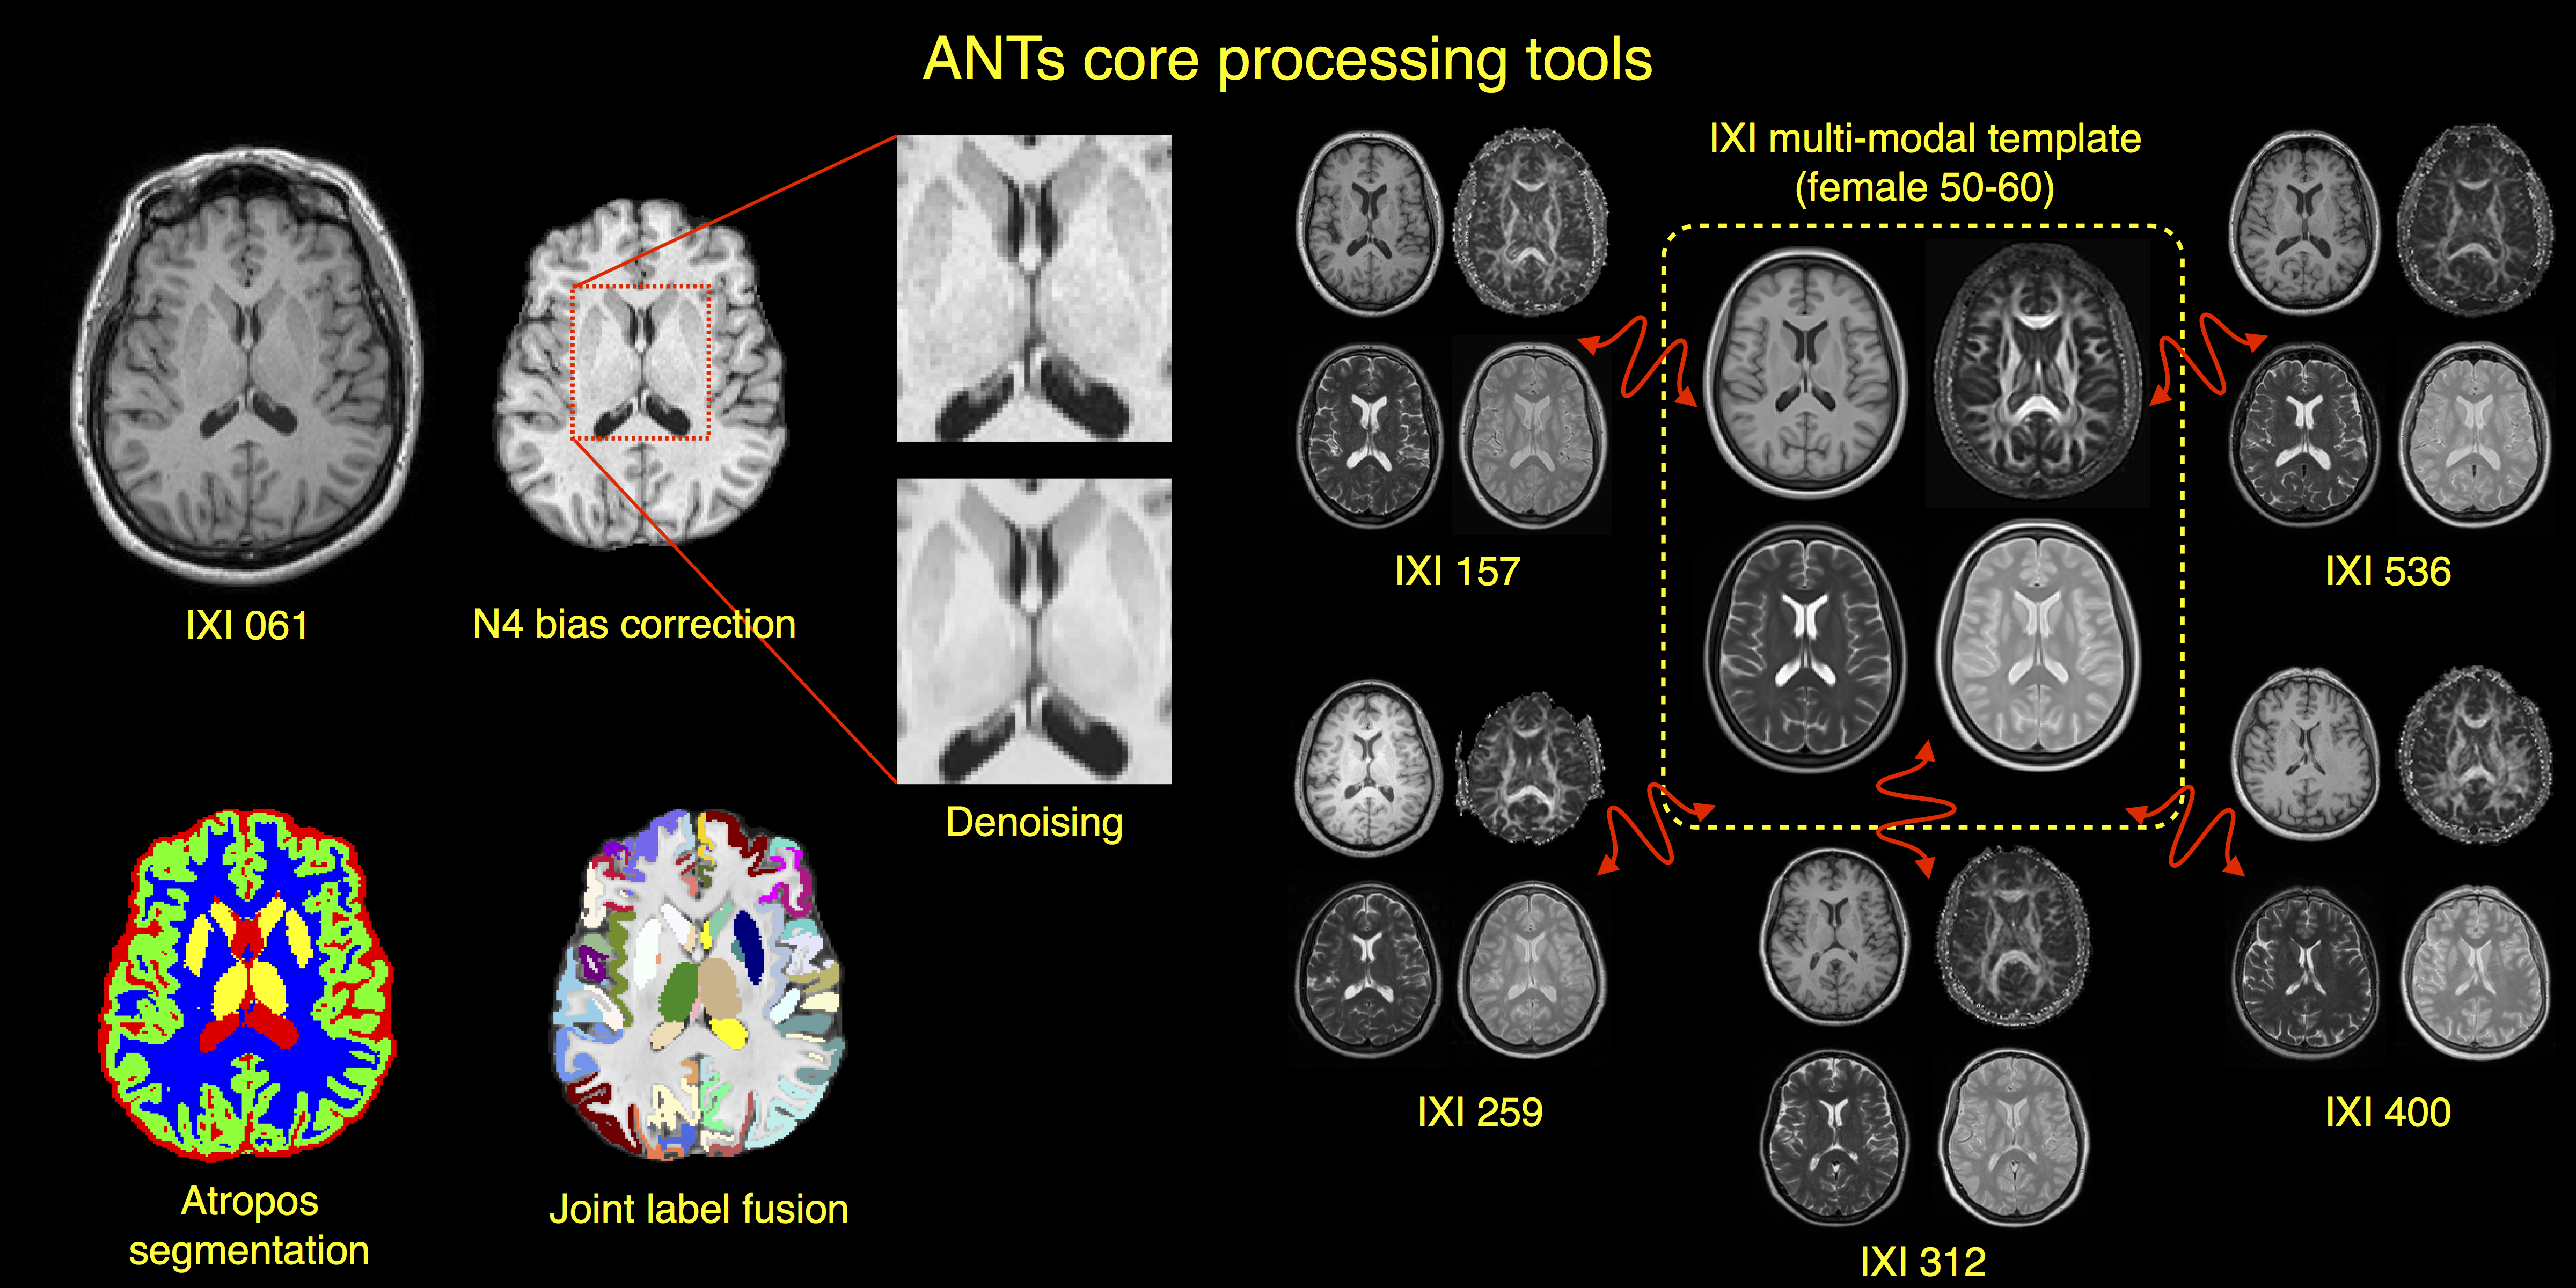
\includegraphics{Figs/coreANtsToolsNeuro.png}
\caption{Core processing tools that have made the ANTs package one of
the most popular neuroimaging toolkits. Fundamental processing tasks
such as image registration, template generation, bias correction,
denoising, intensity-based segmentation, and joint label fusion are
\textcolor{red}{first-in-class} software components which have been
utilized for neuroimaging tasks such as brain extraction and cortical
thickness estimation. \emph{The target applications of these core tools
have an immediate analog for lung-specific tasks such as lung and lobe
segmentation.}}
\end{figure}

\textbf{3(c.1.2) Neuroimaging with ANTs as a model for the pulmonary
community.} ANTs takes advantage of the mature Insight Toolkit in
providing a powerful framework for building scripts and programs to
facilitate processing of large neuroimaging studies. In particular, ANTs
has developed a very large user base by making openly available a
complete suite of fundamental processing capabilities, covering brain
normalization {[}55, 56{]}, brain template generation {[}22{]},
skull-stripping or brain extraction {[}57{]}, prior-based brain tissue
segmentation {[}39{]}, cortical thickness estimation {[}13, 58{]}, brain
tumor segmentation {[}23{]}, and cortical labeling {[}46, 47{]}. These
tools have been wrapped in easy-to-use, well-documented shell scripts
that are accompanied by online self-contained examples with
developer-tuned parameters and are compatible with the major cluster
systems (e.g., SLURM, SGE, and PBS). This project will implement a
similar strategy to support the lung imaging community, as demonstrated
by the following software utilities that have already begun to find
widespread use among pulmonary research groups:

\begin{itemize}
\tightlist
\item
  intra-modal lung registration {[}12{]}
  (\url{https://github.com/ntustison/antsCtLungRegistrationExample}),
\item
  inter-modal lung registration {[}12{]}
  (\url{https://github.com/ntustison/ProtonCtLungMaskRegistration}),
\item
  functional lung segmentation {[}38{]}
  (\url{https://github.com/ntustison/He3LongitudinalAnalysis}), and
\item
  lung and lobe segmentation {[}50{]}
  (\url{https://github.com/ntustison/LungAndLobeEstimationExample}).
\end{itemize}

\begin{figure}[htbp]
\centering
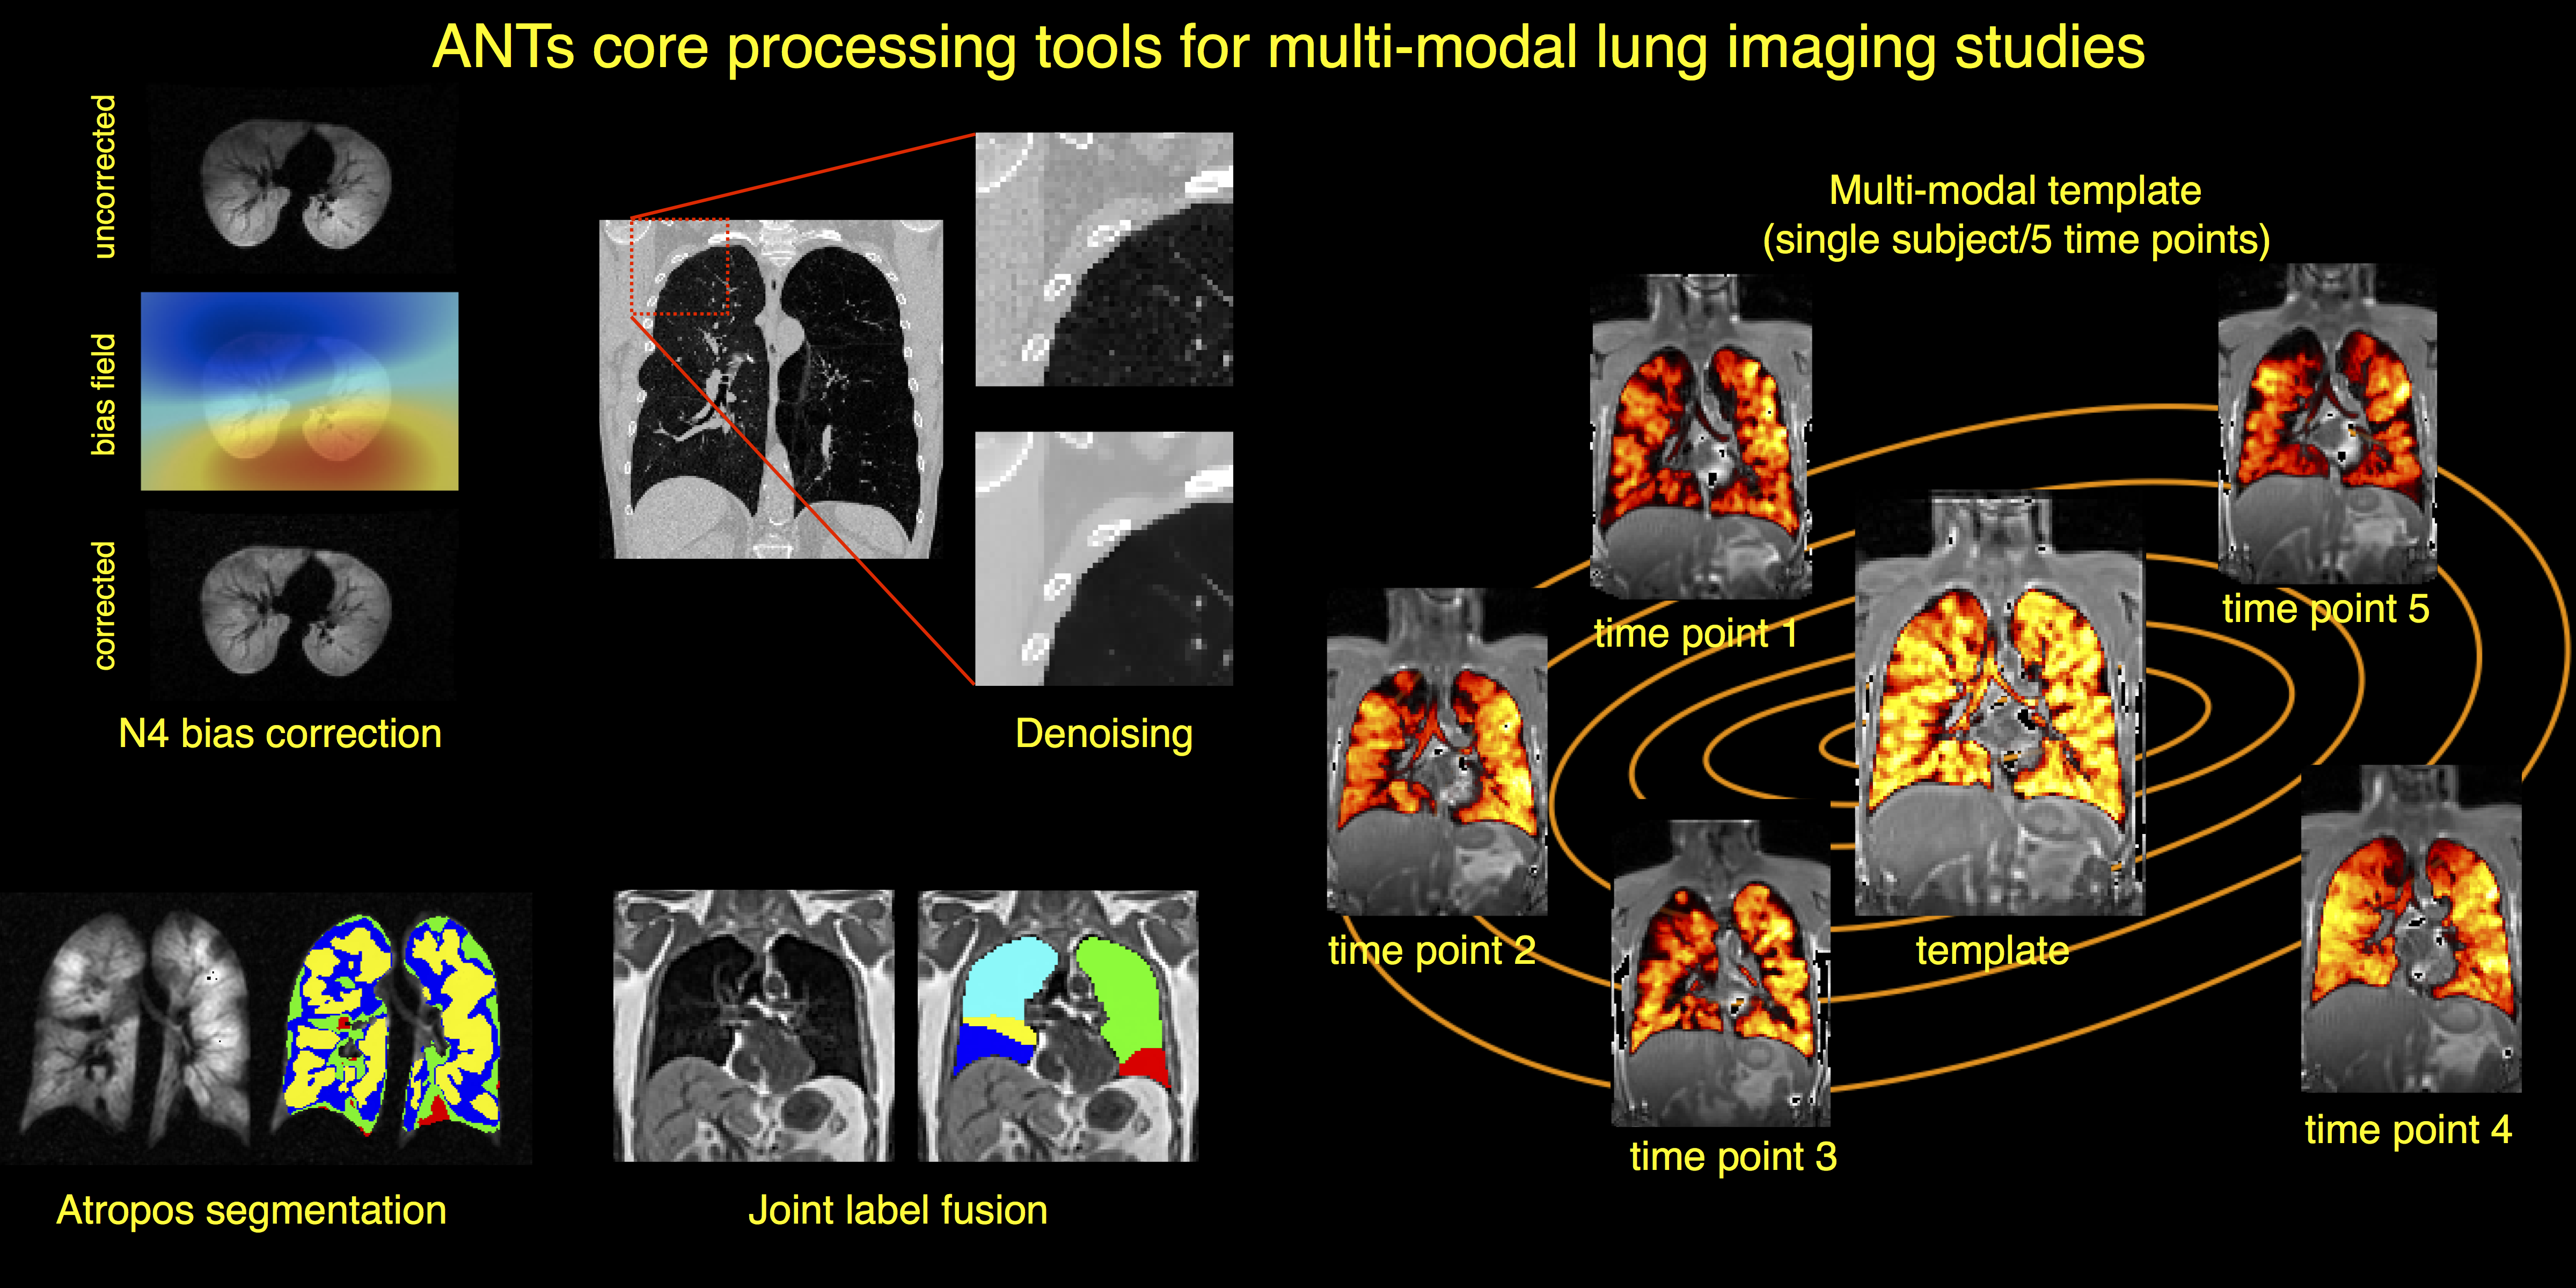
\includegraphics{Figs/coreANtsToolsLung.png}
\caption{ANTs core processing tools for \textcolor{red}{multi-modal}
lung imaging studies. Using ANTs processing tools, our team has
developed several lung-specific extensions such as ventilation-based
segmentation, lung and lobe estimation, and multi-modality pulmonary
template building. Although each of these extensions requires
significant additional development and tuning, a robust and generic
software foundation ensures that these \textcolor{red}{prototypes} are
of high quality and are readily adapted to the pulmonary image domain.}
\end{figure}

\subsubsection{\texorpdfstring{3(c.2) \textbf{Specific Aim 1:} To
develop ITK-Lung, a set of open-source software tools for CT, PET,
\textcolor{red}{and MRI} pulmonary computational
analysis}{3(c.2) Specific Aim 1: To develop ITK-Lung, a set of open-source software tools for CT, PET,  pulmonary computational analysis}}\label{c.2-specific-aim-1-to-develop-itk-lung-a-set-of-open-source-software-tools-for-ct-pet-pulmonary-computational-analysis}

The envisioned open-science tool set for pulmonary image analysis
consists of software, processed data to illustrate the use of the
software, and the ability to evaluate and visualize user-generated
results. With this comprehensive offering, the goal of this project is
to help the pulmonary imaging research community on a much deeper level
than simply providing a set of programs. In order to facilitate
engagement on the part of the community, we are proposing a
multi-faceted approach with ITK-Lung. The main component will be the
core \textcolor{red}{software} tool set described in Sub-Aim 1a which
would permit large-scale processing of multi-modal pulmonary image data.
To illustrate the use of the software, allow for processing of other
public and private data sets, and provide baseline data for algorithmic
comparison, \textcolor{red}{the second
component will involve the release of} CT and 1H MRI annotated atlas
libraries, corresponding templates, and data-generating scripts as
described below. The third component will be significant extensions to
the well-known ITK-SNAP software for an enhanced user experience through
a full featured graphical user interface to support interactive
\textcolor{red}{tuning of parameters and interrogation of processed}
results.

\textbf{3(c.2.1) Sub-Aim 1a will expand the ITK/ANTs open-source
libraries by implementing currently unavailable lung-specific
algorithms.} Many important algorithmic categories implementing
fundamental lung image analysis tasks do not currently exist in any
comprehensive, publicly available package. This is despite the fact that
new algorithms for lung image analysis are frequently reported in the
literature. An extensive survey concentrating on the years 1999--2004 is
given in {[}59{]} which covers computer-aided diagnosis of lung disease
and lung cancer in CT (i.e., detection and tracking of pulmonary
nodules) and provides an overview of the many relevant segmentation
methods for pulmonary structures. Although many algorithms existed at
the time, continued technical development has only increased the number
of available algorithms. However, despite the continued \emph{reporting}
of pulmonary image analysis algorithms, there is no corresponding
increase in algorithmic \emph{availability}. \emph{Additionally, a key
problem in the pulmonary image analysis community is that the lack of
publicly available tools translates directly into a
\textcolor{red}{paucity} of baseline performance standards with which
researchers can compare their own algorithms {[}60{]}. This project
constitutes a specific and overdue response to this major deficiency in
the field.}

\textcolor{red}{
Toward this end, a select set of tools with a track record of good performance, spanning
the range of core functionality and designed to facilitate expansion, will serve the
pulmonary research community
as a well-vetted quantitative resource and baseline for future algorithmic development.}
Table 2 comprises \textcolor{red}{the proposed} functionality for
multi-modal lung \textcolor{red}{image} analysis that would be
incorporated into ITK-Lung in addition to further enhancements to the
registration and segmentation capabilities described in preliminary
work. Using ANTs core tools
\textcolor{red}{with lung-specific modifications,
we have produced prototypical implementations complete with preliminary documentation
and github examples for several of the proposed processing capabilities as described
below.}

\textbf{Atlas-based lung segmentation.} Identification of anatomical
structure in lung images is often a crucial preprocessing step for
quantification of morphological features or ventilation information from
functional images. Quantitative regional analysis typically requires the
\textcolor{red}{delineation} of lung and lobar anatomy. Although much
algorithmic research for lung segmentation has been reported in the CT
literature {[}61{]}, co-opting such technologies is complicated in MRI
by issues such as RF coil inhomogeneity, presence and resolution of
structural detail, and the absence of a physically-based intensity
scaling.

We recently proposed a multi-atlas approach for automatically segmenting
the left and right lungs in 1H MRI {[}50{]}. Multi-atlas approaches to
segmentation have proven highly successful in
\textcolor{red}{multiple domains} {[}46, 52{]}, and these methods
translate readily to pulmonary \textcolor{red}{applications}. Whereas
many current strategies for lung image segmentation employ low-level
processing techniques based on encodable heuristics, consensus-based
strategies, in contrast, optimize the prior knowledge applied to a
specific segmentation problem (cf Figure 2). The evaluation of our
proposed method {[}50{]} demonstrated excellent performance with Jaccard
overlap for the left and right lungs measuring \(0.966\pm0.018\) and
\(0.970\pm0.016\), respectively. Further work for this project includes
extension to CT datasets with a particular emphasis on segmentation in
the presence of lung pathology that will incorporate the data from the
proposed multi-atlas CT library.


\begin{table}[!t]
  \small
   \centering
    \begin{tabular*}{0.75\textwidth}{c @{\extracolsep{\fill}} ccc}
    \toprule
    {\bf Functionality} & {\bf CT} & {\bf 1H MRI} & {\bf 3He MRI}\\
    \cmidrule[1pt](lr){1-4}
    spatial normalization & { \checkmark } & { \checkmark } & { \checkmark } \\
    template generation & { \checkmark } & { \checkmark } & { \checkmark } \\
    lung segmentation & { \checkmark } & { \checkmark } & {  } \\
    lobe segmentation & { \checkmark } & { \checkmark } & {  } \\
    airway segmentation & { \checkmark } & { } & {  } \\
    vessel segmentation & { \checkmark } & { } & {  } \\
    functional segmentation & { \checkmark } & {  } & { \checkmark } \\
    nodule detection & { \checkmark } & {  } & {  } \\
    feature indices & { \checkmark } & {  } & { \checkmark } \\
    \bottomrule
   \end{tabular*}
 \label{table:algorithms}
 \caption{Specific outline of basic functionality proposed for development and evaluation
 in the project
 categorized by modality.  One of the motivations for the collaborative use
 cases as a specific aim is the inevitability that other lung-specific
 algorithmic needs will be identified and will be added to the functionality
 developed and offered as part of this project.  It should also be noted that
 some modality-specific modifications will be required.  For example,
 our lobe estimation approach works well for 1H MRI where no internal anatomical
 features are available for refinement.  This lobe estimation strategy can be directly applied to CT in providing
 spatial prior maps for subsequent subject-specific refinement.
 }

\end{table}


\textbf{Atlas-based lobe estimation.} For regional investigation of
certain lung pathologies and conditions, it is often useful to quantify
measurements of interest within more localized regions, such as the
lobes. However, there is little (if any) usable information in 1H MRI
for image-based lobar segmentation which has led to alternative
geometric subdivisions which are ad hoc, non-anatomical, and do not
adequately address intra- and inter-subject correspondences.
\textcolor{red}{Nevertheless}, we can take advantage of inter-subject
similarities in lobar geometry to provide a prior-based estimation of
lobar divisions using a consensus labeling approach (cf Figure 2).
Specifically, to generate the lobe segmentation in a target 1H or CT
lung image, we register the same-modality atlas set to the target image
(given the general increased robustness of intra-modality
vs.~inter-modality image registration) using the B-spline SyN
registration approach described earlier {[}12{]}. Subsequently, we warp
the set of lobe label images to the target image using the
atlas-to-target transformation. This process will be illustrated
publicly as part of the project using the open-data multi-atlas CT and
1H atlas libraries created as part of Sub-Aim 1b. Since
\textcolor{red}{there is} no intensity information inside the target
lung mask and CT atlas lung masks, a simple majority voting strategy
\textcolor{red}{is used} to generate the \textcolor{red}{consensus}
labeling for the target image. \textcolor{red}{Following this step}, we
remove any labelings outside the lung mask and assign any unlabeled
voxels with the label closest in distance to that voxel.
\textcolor{red}{Additional details can be found} in {[}50{]}, where we
showed that lobar overlap measures in 1H MRI were on par with
\textcolor{red}{methods for CT images  in which} fissure information is
actually visible (left upper: \(0.882 \pm 0.059\), left lower:
\(0.868 \pm 0.06\), right upper: \(0.852 \pm 0.067\), right middle:
\(0.657 \pm 0.130\), right lower: \(0.873 \pm 0.063\)). We will extend
this framework to pulmonary CT in providing spatial prior probability
maps derived from image-specific CT data features such as fissures,
airways, and blood vessels for data-driven, subject-specific lobe
segmentation {[}62{]}.
\textcolor{red}{With the simultaneous acquisition of functional (i.e., PET and 3He images)
and anatomical (i.e., 1H and CT) images, the availability of lobe anatomy estimation
in anatomical lung images facilitates the calculation of regional functional measures which
is difficult to directly obtain from the functional images.}

\textbf{Ventilation quantification.}
\textcolor{red}{The ability to classify} areas of varying degrees of
ventilation \textcolor{red}{represents a basic need in} pulmonary
functional analysis. In {[}38{]}, we presented an automated algorithmic
pipeline for ventilation-based partitioning of the lungs in
hyperpolarized 3He and 129Xe MRI.
\textcolor{red}{Given a whole lung mask (see } \textbf{Atlas-based lung
segmentation}),
\textcolor{red}{the original pipeline performs MR inhomogeneity correction followed by
Bayesian segmentation with an MRF prior.} Without ground truth data for
evaluation, we used a consensus labeling approach {[}63{]} to
simultaneously estimate the true segmentation from given ``raters''
\textcolor{red}{and the performance of those raters with respect to that estimation.
In this evaluation, "raters" refers to the segmentation from our automated approach
and the manual tracings of three trained individuals.} In terms of
combined specificity and sensitivity, our algorithm demonstrated
superior performance with the added benefit of being reproducible and
less time-consuming.
\textcolor{red}{Future enhancements to this pipeline will include the incoproration
of 1) an iterative bias-correction/segmentation scheme that should yield improved
optimization solutions and 2) a better performing denoising protocol based on the patch-based
method} described in {[}51{]}.

\textbf{Multi-modality lung template construction.}
\textcolor{red}{Because} the template construction algorithm described
in {[}22{]} \textcolor{red}{was
originally developed for proton MRI and neuroimaging applications, it will be
modified in this project to additionally admit CT and PET data and further
adapted for specialized use in studies of the lung.
The latter development will build on our recent} innovations in
diffeomorphic registration technology \textcolor{red}{that} has led to a
Symmetric Normalization B-spline variant which will be extended and
refined to include patch-based similarity metrics suitable for
minimizing the computational footprint of
\textcolor{red}{problems involving very large images of the kind commonly
encountered in lung studies while at the same time} providing accurate
normalizations {[}12{]} for pulmonary data {[}21{]}.
\textcolor{red}{For functional lung imaging data (i.e., PET and 3He), this
step generates the statistical coordinate system which could be used for subsequent
voxelwise analyses to determine local correlation with clinical measures.}

\textbf{Feature indices.} Imaging biomarkers for characterizing
emphysema in CT have have been well researched, although there are ample
opportunities to refine these methods as well as to introduce more
advanced approaches. Examples of the latter include texture analysis for
identifying the centrilobular and ground-glass opacities and fractal and
connectivity approaches to differentiate centrilobular from panlobular
emphysema. The available indices for CT image analysis can roughly be
divided into those that characterize the pulmonary parenchyma:
volumetric tissue (e.g., {[}64, 65{]}), distribution of low attenuation
areas (LAA) (e.g., {[}66, 67{]}), cooccurrence and run-length matrix
features (e.g., {[}68, 69{]}), attenuation statistics (e.g., {[}70,
71{]}), deformation measures (e.g., {[}72, 73{]}), and stochastic
fractal dimension features (e.g., {[}68, 71{]}); and those that
characterize the airways (e.g., {[}74--76{]}). The former are important
for subjects with an emphysematous component of disease, whereas the
latter are important for subjects with a bronchitic
\textcolor{red}{disease} component.
\emph{\textcolor{red}{An important benefit of this
project's multi-modality scope} is that many of these measurements can
also be directly applied to discriminative analysis using 3He MRI
\textcolor{red}{and PET} for a variety of lung diseases.
\textcolor{red}{Moreover}, recent work has demonstrated {[}77{]} these
indices can \textcolor{red}{additionally} be studied not only at any
particular single time point, but also for changes with time.}

\textbf{Airway segmentation.} \textcolor{red}{Lung} airway morphology
has been previously utilized as a biomarker for disease characterization
but there are many other potential uses motivating the inclusion of
airway segmentation in any pulmonary image analysis toolkit. In an
evaluation of 15 airway segmentation algorithms {[}78{]} for the
Extraction of Airways from CT challenge held in 2009, the top 2
performers were the algorithms of {[}79{]} and {[}80{]} with the latter
being one of the more conservative algorithms and the former being more
prone to false positives. Our plan is to provide an implementation of
{[}79{]} which employs a sharpening of the airway branching edges and
\textcolor{red}{the use of} adaptive cuboid volumes to
\textcolor{red}{realize} a region-growing airway segmentation approach.
We \textcolor{red}{will then} augment this functionality with
complementary aspects of our previous work {[}81{]} for removing leakage
path candidates.

\textbf{\textcolor{red}{Vessel segmentation.}}
\textcolor{red}{In contrast to much of what is described in the literature, there exist
key contributions for pulmonary vessel segmentation available to the public, specifically
the algorithms described in} {[}82{]}.
\textcolor{red}{Similar to much of the
research for enhancement of vessel-like morphology in different anatomies, the authors
employed Hessian-based filters for deriving a ``vesselness'' function.
Their approach ranked consistently among the top performers in the
VESSEL12 challenge organized in conjunction with the IEEE International Symposium on
Biomedical Imaging (ISBI 2012).  Given that the first author is a regular
ITK contributor, the corresponding code will be easily integrated into our platform.
}

\textbf{\textcolor{red}{Perfusion analysis.}}
\textcolor{red}{A nonparametric deconvolution technique for quantifying cerebral blood
flow was first presented in} {[}83{]}
\textcolor{red}{and subsequently extended for use in assessing
pulmonary blood flow} {[}84,
85{]}\textcolor{red}{.  This deconvolution strategy was recently
implemented by our group for a separate lung imaging study but will be modified for this
project to automatically select the arterial input region and volume of interest.}

\textbf{\textcolor{red}{Graphics processing unit acceleration.}} In
preliminary work, we have successfully used OpenGL shader language to
perform image processing operations, such as computation of similarity
metrics between images or extraction of features from images, on the
graphics processing unit (GPU) at real-time speed. GPU requirements for
ITK-Lung will be very modest and would be met by virtually any mid-range
desktop computer sold today (e.g., a mid-range iMac). We plan to
integrate both affine and deformable registration with GPU acceleration
into ANTs. The three components of diffeomorphic deformable registration
in ANTs that account for over 95\% of computation time are: 1)
computation of the gradient of the similarity metric (e.g., mutual
information, cross-correlation); 2) smoothing of the gradient using
Gaussian kernels; and 3) image and vector field interpolation. All three
components are highly parallelizable, and we will write OpenGL shader
code for performing these operations on the GPU, analogous to the code
currently used for metric computation in GPU-based affine registration
in ANTs.

\textbf{\textcolor{red}{Computational power.}} With the proposed GPU
acceleration of image registration, we expect that even the most complex
registration-dependent problems will be possible to solve on a desktop
computer in under 10 minutes. \textcolor{red}{This estimate is based on}
preliminary work \textcolor{red}{in which} we have developed a CPU-based
accelerated version of the ANTs deformable registration algorithm that
is approximately 15 times faster in typical problems than the version
currently in use. This means that on a typical 8-core CPU, the same
registration of
\textcolor{red}{$512 \times 512 \times {\sim}500$ voxel images} can be
\textcolor{red}{completed in under 20 minutes
instead of the 1-2 hours it would take on a single CPU core using the current production version of ANTs.}
This dramatic improvement was made primarily though 1) use of more
efficient metric gradient computation algorithms, 2) use of single
instruction multiple data (SIMD) parallelization on Intel CPUs, and 3)
extensive code profiling and optimization. With the move to the GPU, we
expect to speed up registration by another factor of 4--5 times.
Therefore, the vast majority of ITK-Lung users will not need to have
access to high-performance computing clusters or other expensive
hardware.

However, for power users with very large datasets or datasets that
require more compute-demanding parameters or higher-resolution
registration, we will also provide an alternative offline processing
mode, in which the registration tasks are executed on an external
high-performance computing resource. In this mode, the ITK-Lung GUI (see
Sub-Aim 1c) will provide a user interface front-end to
\textcolor{red}{available processing pipelines} running remotely. It
will send data to the external resource over the network, monitor and
control pipeline execution, and receive results when processing is
complete. This remote pipeline execution mode will additionally support
other highly computationally intensive tasks \textcolor{red}{as well as}
other data processing tasks that may be added in the future. The
external resource may be either a physical Linux cluster or a virtual
one hosted on the Amazon Web Services (AWS) cloud. For AWS, we will use
the MIT StarCluster software (\url{http://star.mit.edu/cluster}) to
launch a virtual cluster directly from the ITK-Lung GUI on demand. We
will take advantage of the GPU enabled AWS instances,
\textcolor{red}{which would allow} the speed-ups described above to be
combined with parallel execution across multiple hosts. The advantage of
using AWS is that a power user would not need to purchase and configure
expensive hardware---they just register for an AWS account. While this
would incur costs for computational time used, these costs would be a
fraction of the cost of the required hardware. For instance, even with
the most demanding datasets and parameters,
\textcolor{red}{it is hard to envision a processing task that would require
more than an hour when distributed across 40 GPUs on AWS, the cost of which is currently \$26.}
Data transfer to AWS will incur negligible costs (\$0.01 per GB),
particularly since data may be uploaded at reduced resolutions
sufficient for many processing tasks.

\textbf{3(c.2.2) Sub-Aim 1b will provide two annotated multi-atlas
libraries, one for CT and another for 1H MRI.} The corresponding group
templates will also be provided along with the scripts to produce the
results using ITK-Lung. As a complement to the open-source software
provided in Sub-Aim 1a, we will generate atlas libraries for both CT and
1H MRI acquisitions.
\textcolor{red}{As indicated above, the availability of such atlases as anatomical priors
is prerequisite to application of the current state-of-the-art in robust and accurate lung
and lobe segmentation within their respective modalities.} Additionally,
the accompanying annotations provide an open-data platform for
quantitatively assessing other lung and lobe segmentation algorithms.
Both libraries will consist of \(n=30\) different subjects to represent
a range of lung size and shape. The CT atlas library will include lung,
lobe, airway and vessel segmentations, \textcolor{red}{whereas t}he 1H
MRI atlas library will include left/right lung segmentations and lobar
estimations {[}50{]}. Along with the annotated data we will provide the
scripts and documentation to allow \textcolor{red}{independent}
reproduction of the ITK-Lung results. \textcolor{red}{Finally, optimal}
group templates {[}22{]} for the two atlas libraries
\textcolor{red}{will be generated and made openly available to be utilized as common coordinate
frameworks to support voxelwise analyses.}

\textbf{3(c.2.3) Sub-Aim 1c will develop a graphical user interface
(GUI) for running ITK-Lung on user data and evaluating processed
results.} ANTs will be the workhorse toolkit for the registration
development effort in Aim 1, and the creation of a user-friendly GUI
enabling interactive access for the first time to ANTs functionality
will be a critical innovation toward a comprehensive registration
solution for \textcolor{red}{multi-modality} imaging studies of the
lung. The existence of the GUI will not only open ANTs to users without
programming experience---which is expected to greatly expand its already
considerable user base and in turn further increase its impact on the
field---but will also significantly enhance the power of ANTs by
allowing human/expert input to interactively tune parameters and
intelligently initialize as well as steer the registration toward the
solution that best satisfies both user and algorithmic constraints.
Equally important, the GUI will permit qualitative and quantitative
assessment of the results produced by ITK-Lung as well as potentially
other software, another much needed capability not currently available
to the general community. \textcolor{red}{Taking} these considerations
\textcolor{red}{into account}, we propose to base the GUI front-end to
ITK-Lung on the ITK-SNAP multi-platform, open-source tool for
interactive user-guided medical image segmentation and data
visualization {[}86{]}, \textcolor{red}{the development of which} is led
by project investigator Paul Yushkevich. ITK-SNAP provides an effective
combination of semi-automatic segmentation functionality based on active
contours {[}87{]} and manual delineation functionality, put together
into a compact and easy-to-learn GUI, that perfectly complements the
automated segmentation functionality proposed for development in this
project. ITK-SNAP design emphasizes interaction and ease of use, with
the bulk of the development effort dedicated to the user interface. ITK-
SNAP has thousands of users (there have been over 2000 downloads per
month in the last year), and our 2006 paper on ITK-SNAP {[}86{]} has
been cited over 1400 times (Google Scholar) in the context of various
biomedical domains. ITK-SNAP will also be used in this project for
manual labeling of the proposed lung atlases; it is already used for
this purpose by many investigators. \emph{Most crucially, we believe
that our track record with ITK-SNAP as well as ANTs demonstrates our
team's commitment to producing high-quality research software and making
it accessible to the wider research community through open-source
practices, intuitive user interfaces, and outreach efforts. These
strengths of the team will be applied to the software and data developed
in the course of this project.}

Several features will be added to ITK-SNAP to enhance visualization and
quantitation for the registration and segmentation results of the
lung-specific algorithms developed in the project. Users will be able to
edit and annotate these segmentations, modify registration transforms,
and extract quantities both globally and regionally. Transforms will be
modifiable via manual annotations (clicking corresponding landmarks,
tracing curves, and/or painting regions) or by directly modifying
transform parameters. Quantitative parameters, such as volumes and
strain tensors, will be available through the ITK-SNAP interface.
Finally, existing ITK-SNAP functionality for segmentation visualization
will be \textcolor{red}{expanded} to support evaluation of registration
quality, including a dashboard of performance metrics, linked cursors
identifying corresponding positions in multi-window configurations, and
fused data displays with adjustable blending. \emph{These proposed
enhancements to the software will be extremely useful to the general
imaging research community and not just those investigators targeted in
this project. Thus, the impact of this work will be both immediate and
broad on pulmonary-driven science and research.}

\textbf{3(c.2.4) Software engineering.} Both ANTs and ITK-SNAP
development, based on a solid foundation provided by the Insight
Toolkit, utilizes open-source software engineering best practices, such
as the use of Git version management software for collaborative
development and easy branching and merging; use of a centralized
repository (SourceForge) for code, executable and data sharing; and use
of the CMake/CTest/CDash suite for cross-platform development, testing
and automatic builds. Virtual machines with different versions of
Windows, MacOS and Linux operating systems generate nightly builds and
execute test code, uploading a binary to the central SourceForge
repository. ANTs and ITK-SNAP are documented through video and text
tutorials, housed online on dedicated websites {[}11, 89{]}. A similar
infrastructure will be developed for the software resources proposed in
Aim 1.

\subsubsection{\texorpdfstring{3(c.3) \textbf{Specific Aim 2.} Validate
and disseminate the developed ITK-Lung resources by leveraging use cases
from a broad network of partner investigators representing the
state-of-the-science in lung imaging
research}{3(c.3) Specific Aim 2. Validate and disseminate the developed ITK-Lung resources by leveraging use cases from a broad network of partner investigators representing the state-of-the-science in lung imaging research}}\label{c.3-specific-aim-2.-validate-and-disseminate-the-developed-itk-lung-resources-by-leveraging-use-cases-from-a-broad-network-of-partner-investigators-representing-the-state-of-the-science-in-lung-imaging-research}

This aim builds on the project team's long and successful track record
of collaboration with the general user community. In particular, the
investigator-driven studies presented below are carefully selected both
for their capacity to fully exercise the developed tools and to provide
a comprehensive representation of the various processing and analysis
tasks of interest to the community.
\textcolor{red}{Two evaluation groups will serve as primary and secondary beta testers, respectively:
institutional and external collaborators.  For the former, the development team will be embedded in
the labs of project co-investigators, providing training to lab personnel and assisting with the
creation of customized analysis pipelines.  These experiences will be used to develop tutorial
materials and processing examples that our external collaborators will independently test by
processing their own data in-house with beta versions of the proposed software and data resources.
Similarly, the dissemination and user support mechanisms outlined in the Resource Sharing Plan will
be refined by employing these as much as possible to communicate and interact with the external
collaborator group.}

\subsection{Institutional
collaborators}\label{institutional-collaborators}

\textbf{3(c.3.1) Novel imaging biomarkers for Chronic Obstructive
Pulmonary Disease (COPD).} Co-investigator \textbf{Mike Shim} and his
group have been actively developing 3D hyperpolarized xenon-129
dissolved-phase MRI (HXe MRI) as a sensitive biomarker for accurately
characterizing phenotypes and severity of COPD. This protocol permits
regional mapping of ventilation and gas uptake by tissue and blood in
human lungs with single breath hold {[}90--92{]}. This project plans to
establish connectivity between these advanced HXe MRI imaging signatures
and important clinical outcomes of COPD to advance HXe MRI as a novel
clinical diagnostic tool. This new biomarker tool will naturally lead to
deeper mechanistic understanding of COPD at the molecular-physiologic
and clinical levels and support identification of potential
pathophysiologic derangement associated with COPD and a new method to
accurately predict therapeutic response to current standard COPD
therapies. Refinement of HXe MRI as a pulmonary diagnostic tool is
anticipated to encourage development of new clinical interventions.

HXe MRI is the first non-invasive imaging technique that can provide
regional information about three unique characteristics of lung
function: lung ventilation, size and connectedness of distal alveolar
airspaces, and HXe gas transfer from airspaces to red blood cells. HXe
MRI, therefore, is anticipated to overcome the limitation of pulmonary
function testing (PFT) which only provides physiologic parameters of the
lung as a whole unit, and High Resolution CT (HRCT) which only provides
anatomic characterization without physiologic information. HXe MRI has
potential to detect pathologic changes present in COPD patients with
high sensitivity and specificity previously unattainable by the current
clinical standard (PFT and HRCT). Moreover, HXe MRI can determine
whether gas transfer abnormalities are due to impaired ventilation or
reduced gas-exchange, and thus provide new insights into the
pathogenesis of COPD in individual patients.

Crucial to the success of establishing the utility of HXe MRI as a
sensitive biomarker for accurately characterizing COPD phenotypes is
quantification of imaging signatures in an automated and robust fashion.
Identification of ventilation dead space (\(V_D\)) for correlation with
GOLD classification will utilize the ventilation-based segmentation
functionality in ITK-Lung {[}38{]}. In order to determine lobar values
of HXe MRI, this study will utilize the recently proposed lobar
estimation algorithm {[}50{]} that will be available for both proton MRI
and CT.

\textbf{3(c.3.2) Hyperpolarized gas imaging in children with asthma.}
Advances in rapid image sequencing methods have facilitated the
acquisition of high-quality hyperpolarized gas MR images in pre-school
children {[}93{]}. Furthermore, improvements in image processing and
signal intensity analysis have made possible accurate measurements of
lung volume compartments {[}38{]}. Co-investigators \textbf{Gerry
Teague} and \textbf{Talissa Altes} are applying these innovations in
children with asthma to study whether the lung defect volume \% as
measured by hyperpolarized lung MRI correlates with a range of clinical
features. They hypothesize the ventilation defect volume \% would be
higher in children with severe asthma, and correlate not only with the
degree of airflow limitation, but indicators of asthma control,
treatment, and inflammation.

Precise measurement of ventilation volumes by hyperpolarized noble gas
MRI not only has the potential to resolve the spatial and temporal
characteristics of gas distribution in children with asthma, but could
also expand clinically relevant information in regards to asthma
severity and its features. In the past, simple computer-assisted systems
{[}94{]} or hand counts of visual defects were used to estimate the
ventilation defect volume {[}95{]}. Development of more advanced
techniques (in terms of acquisition and analysis) will facilitate rapid
conversion of complex hyperpolarized gas signal data into volume
compartments for clinical applications.

Absolutely crucial to the advanced techniques being developed by
Dr.~Teague and his group are sophisticated image analysis tools like the
ones being proposed in this project. For example, our ventilation-based
segmentation method is already being used to determine volumetric
compartments based on lung function. Additional ``cleaning'' necessary
for these data include denoising techniques {[}51{]} implemented and
made available in ANTs. Lobe estimation will be possible by refining the
techniques originally described in {[}50{]}.

\textbf{3(c.3.3) Characterization of COPDGene cohort by hyperpolarized
gas (HP) MRI.} Co-investigator \textbf{Rahim Rizi} is leading a study of
lung function and structure in COPD using HP MRI. Once inhaled, this gas
can tell the researcher how well specific lung regions replace the air
during the normal breathing cycle (Fractional Ventilation, FV), how much
oxygen is in the airspaces (Oxygen Tension, PAO2), and if the normal
spongy tissue structure has been compromised in lung disease (Apparent
Diffusion Coefficient). Subjects will include those at risk for lung
disease, and those displaying mild and moderate COPD. They will be
mostly drawn from the well-characterized population currently enrolled
in the COPDGene trial (10,000 subjects overall) such that standard
clinical images (End Inspiration and End Expiration CT) and Pulmonary
Function Tests (PFTs), as well as genetic sequencing, will already have
been done. Each subject will be imaged twice during the course of the
five-year study, and regional features will be compared between the CT
and MRI images to the genetic markers, changes in clinical measurements,
and patient quality of life.

The proposed study will generate non-invasive biomarkers of COPD
progression derived from minute, short-term alterations in lung function
and microstructure. Due to the excellent safety profile of MRI, these
metrics will be appropriate for use in novel, flexible study designs.
Perhaps most importantly, this research will enhance understanding of
the natural history of COPD. In doing so, it will provide a vital
supplement to ongoing efforts to identify COPD subtypes by adding
substantial physiologic detail to descriptions of this disease. The
overall goals of the study experiments are: a) to develop imaging
markers that better identify early COPD; b) to develop tests that
predict health deterioration due to COPD; c) to determine if specific
patterns of disease progression are associated with genetic markers
identified in the larger COPDGene study; and d) to determine if disease
progression is in part caused by excessive stretch in regions of the
lung next to blocked-off areas unable to inflate normally.

More than 200 million people suffer from COPD worldwide. Yet effectively
assessing the progression of this increasingly prevalent disease and
monitoring its response to treatment remain problematic. Hyperpolarized
gas MRI can help rectify these issues by providing sensitive
measurements of lung physiology and microstructure, but its adoption by
clinicians and investigators has been slow. In contrast, CT-based
methods for measuring emphysema, airway wall thickening, and expiratory
air trapping have become common in COPD clinical studies. There are
several reasons for this: CT is more accessible, its images possess
excellent spatial resolution, and quantification of these images is
currently superior. However, most CT-based parameters have only an
indirect relation to physiology, and the modality exposes patients to
ionizing radiation. Both of these shortcomings can be addressed by HP
gas MRI. Consequently, the study seeks to more fully exploit the
clinical potential of HP gas MRI by optimizing and testing parameters
for the regional assessment of COPD patients and symptomatic smokers.

A novel multi-breath HP MRI technique allows for the simultaneous
measurement of fractional ventilation (FV), regional partial pressure of
oxygen (PAO2), and apparent diffusion coefficient (ADC). Obtaining all
three parameters in a single scan reduces the necessary amount of
imaging gas while increasing accuracy by correcting artifacts associated
with collateral ventilation and the slow filling of parenchyma in
diseased lungs. Each of these metrics allows for the investigation of a
vital aspect of lung disease progression and their comparison with the
current CT-based standard of care will help to more clearly understand
different features and phenotypes of COPD.

The proposed image analysis software will be central to the successful
conduct of the following tasks necessary to establish the goals of this
study:

\begin{itemize}
\tightlist
\item
  Registration of the multibreath/multislice gas MRI images of the whole
  lung consisting of a minimum of seven time points
\item
  Registration and analysis of inspiratory and expiratory CT for airway
  changes to assess airway collapsibility and remodeling and other CT
  markers
\item
  Registration and analysis of inspiratory and expiratory CT with MRI to
  study the similarities and differences of the two modalities in
  phenotyping the COPD population
\item
  Registration of the follow-up MRI and CT images (two years) to
  determine if disease progression is in part caused by excessive
  stretch in regions of the lung next to blocked-off areas unable to
  inflate normally (based on the baseline MRI and CT)
\end{itemize}

\textbf{3(c.3.4) Advanced image analysis of CT for early diagnosis and
prognosis of bronchiolitis obliterans syndrome (BOS) in lung transplant
patients.} Co-investigators \textbf{Eduardo Barbosa} and \textbf{Warren
Gefter} are conducting a retrospective study of more than 300 lung
transplant patients to advance the early diagnosis of BOS. Lung
transplantation is an established treatment for end-stage, irreversible
pulmonary disease, particularly due to COPD and interstitial lung
disease (ILD). While continued improvements in surgical techniques and
immunosuppressive medications have reduced the complication rates and
increased short-term survival after the procedure, chronic allograft
rejection due to bronchiolitis obliterans (a fibrous obliterative
disease of bronchioles representing the histological hallmark of chronic
rejection and resulting in obstructive pulmonary physiology) remains the
major cause of morbidity and mortality after six months following
transplantation. Bronchiolitis obliterans currently represents the
greatest limitation to long-term survival after lung transplantation.
While the diagnosis of bronchiolitis obliterans is a pathologic one and
therefore requires invasive biopsy, the distribution of disease is
patchy, with focal areas of abnormality surrounded by normal lung, and
consequently even biopsies may fail to demonstrate the diagnosis. For
these reasons, the International Society for Heart and Lung
Transplantation has recommended using declining spirometry, termed
bronchiolitis obliterans syndrome (BOS), as a surrogate marker of
chronic allograft rejection. In clinical practice, the diagnosis of BOS
is suspected based on an unexplained decline in lung function (measured
by PFT, of greater than 20\% of baseline FEV1) and worsening cough and
dyspnea, in the absence of other explanations such as pulmonary
infection or congestive heart failure. MDCT plays an important role by
demonstrating low attenuation areas representing air trapping,
particularly on expiratory images, which correlate with the presence of
bronchiolitis obliterans. Prior studies reported limited sensitivity for
the early diagnosis of bronchiolitis obliterans; however these utilized
semi-quantitative or qualitative assessment of air trapping in
non-volumetric data sets. This study aims to assess whether more
advanced, fully automated imaging analysis can detect early BOS prior to
development of clinically apparent disease.

PFT is the current reference standard for diagnosis of BOS; however, by
the time PFT abnormalities beyond the threshold of BOS diagnosis ensue,
the disease is already manifest and is not reversible with existing
therapies. It is conceivable that sophisticated analysis of CT,
including quantitative attenuation masks in inspiratory and expiratory
datasets, image registration and texture based feature extraction {[}96,
97{]} may allow earlier detection of BOS in the preclinical phase,
potentially generating surrogate biomarkers for drug trials and earlier
prognostication.

Application of the proposed advanced software tools and algorithms in
this project for quantitative analysis of CT images in lung
transplantation patients will be crucial to enable computation of an
array of first and second order statistics \textcolor{red}{that} would
capture not only attenuation maps but also regional deformation and
texture based features. In combination, this would allow multiparametric
statistical modeling that may predict which patients will develop BOS
before PFT abnormalities beyond the diagnostic threshold ensue. Such
tools will be extended to other diffuse lung diseases, potentially
generating new biomarkers for diagnosis, prognostication, and
therapeutic trials.

\textbf{3(c.3.5) Novel PET/CT biomarkers for early prediction of
treatment response and survival in patients with non small cell lung
cancer (NSCLC).} PET and CT have traditionally played important roles in
diagnosis, staging, and predicting treatment response in NSCLC
{[}98--100{]}. Although many studies have demonstrated diagnostic and
prognostic value of tumor metabolic burden and morphological information
derived from PET/CT imaging measures {[}100, 101{]}, current ability to
predict treatment response and survival following radiation therapy in
NSCLC is far from satisfactory {[}102{]}. The poor performance of
existing methods may be due to a number of reasons: first, most studies
have been limited to primary tumor lesions and ignored the information
available in other lesions/regions {[}103{]}; second, many
investigations have focused on global image measures of tumors, such as
those derived from standardized uptake value (SUV) of PET images and
tumor morphological information, which may not be sufficient for
capturing subtleties of tumor characteristics and tumor heterogeneity
{[}104, 105{]}; and finally, group-level statistical analysis strategies
are typically adopted to evaluate imaging markers, which may not be
effective for personalized prediction {[}106{]}.

To improve prediction of radiation therapy treatment response and
survival in patients with NSCLC based on PET/CT imaging data,
co-investigator \textbf{David Mankoff} and collaborators are developing
methods to adaptively extract image features from the data that are then
input into a multi-task learning framework constructed to jointly model
(and leverage potential statistical correlations between) the problems
of predicting treatment response and survival. The proposed software
tools will fulfill essential pre-processing needs of the study: PET/CT
data will be co-registered and a wealth of image features calculated
using ITK-Lung.

\subsection{External collaborators}\label{external-collaborators}

\textbf{3(c.3.6) Comparison of automated multi-modality registration
methodologies to manual registration for assessing lung CT bronchial
morphologic changes and hyperpolarized helium MR ventilation defects in
asthma patients: Can automation speed the work flow for combining
structure and function using airways measures from CT and ventilation
measures from HP gas MRI?} Our collaborators \textbf{Sean Fain} and
\textbf{Mark Schiebler}, \textbf{University of Wisconsin}, are part of
the SARP (Severe Asthma Research Program) team developing imaging
biomarkers of asthma severity for predicting asthma exacerbation. The
approach of finding airway abnormalities that correlate with ventilation
defects is viable only with the availability of robust image
registration across the two modalities. Furthermore, translation to the
clinic will require standardized implementations across sites, and the
project's open-source platform is ideal for this purpose.

\textbf{3(c.3.7) Validation of voxel-based ventilation CT.} Our
collaborator \textbf{Jim Wild}, \textbf{University of Sheffield}, has
been active in the field of methods development for quantitative
pulmonary imaging and its clinical translation for more than a decade.
Relevant to this project, his group requires advanced registration
capabilities to validate a novel CT technique for obtaining
high-resolution images of pulmonary ventilation. In addition, there is
need within his research for multi-modality registration of pulmonary CT
and MRI images as well as segmentation of key lung structures as part of
standard processing workflows.

\textbf{3(c.3.8) Deep functional phenotyping of COPD.} Our collaborator
\textbf{Hans-Ulrich Kauczor}, \textbf{University Medical Center
Heidelberg}, is leading the COSYCONET (German COPD and Systemic
Consequences--Comorbidities Network) study, the world's first
prospective multicenter trial comparing proton MRI and CT imaging for
characterizing COPD, with the latter modality serving as the reference
standard. Automated image registration and segmentation will play a
vital role in defining the quantitative CT (air trapping, airway
collapsibility and remodeling, and pulmonary blood volume and vascular
pruning) and MR (air trapping, perfusion volume defects, and hypoxic
vasoconstriction) imaging biomarkers that form the basis for the study.

\textbf{3(c.3.9) Longitudinal imaging follow-up in COPD and lung
cancer.} Our collaborator \textbf{Joon-Beom Seo}, \textbf{Asan Medical
Center}, directs the imaging component of the Korean Obstructive Lung
Disease (KOLD) cohort study, which has collected over 1000 COPD cases
from 17 participating centers with repeated imaging since 2005. He also
leads a national lung cancer radiomics project that has accrued 800
cases to date. In both studies, robust image registration is essential
to tracking changes over time, and segmentation is an additional
requirement to support automated lesion delineation for the cancer
project.

\textbf{3(c.3.10) Advanced image processing pipelines for MR
image-guided pulmonary therapy decisions and support.} Our collaborator
\textbf{Grace Parraga}, \textbf{University of Western Ontario}, has been
at the forefront of MR imaging of lung structure and function since
2005. A major challenge hampering widespread translation of current
pulmonary imaging advances is the lack of precision in their
interpretation, thereby complicating the planning and guiding of
targeted therapies. The project's software tools will enable the
development of robust analysis pipelines for the translation of in vivo
imaging biomarkers in an open and consistent manner across platforms and
centers. This work, carried out in collaboration with industrial
partners, will support patient phenotyping and stratification to therapy
as well as measurement of longitudinal changes and response to therapy.

\textbf{3(c.3.11) Functional MR imaging of the lungs using
hyperpolarized and inert gases.} Our collaborator \textbf{Mitchell
Albert}, \textbf{Thunder Bay Regional Research Institute}, has been
advancing the use of inert fluorinated gases that can be breathed
continuously in order to measure indicators of wash-in, wash-out and air
trapping with dynamic imaging protocols. To compute the wash-in and
wash-out time constants on a pixelwise basis, access to accurate and
reliable image registration tools will be essential.

\textbf{3(c.3.12) Multimodality imaging studies of pulmonary diseases.}
Our collaborator \textbf{Edwin van Beek}, \textbf{University of
Edinburgh}, has been conducting various multimodality studies, including
the evaluation of pulmonary fibrosis using both gadolinium-enhanced MRI
and contrast-enhanced CT perfusion imaging, and the assessment of lung
nodules using PET-CT and CT perfusion imaging. These relatively new
techniques would benefit from quantitative analysis of contrast
enhancement, and advanced image registration and segmentation
capabilities will both be necessary toward this end.

\textbf{3(c.3.13) Computational imaging biomarkers for diverse thoracic
malignancies.} Our collaborator \textbf{Yoshiharu Ohno}, \textbf{Kobe
University}, leads a comprehensive program of multi-modality imaging
(CT, MRI, PET, molecular imaging) research on lung cancer, COPD, ILD,
and pulmonary infectious diseases. His myriad image analysis needs
include quantitative characterization of: lung parenchyma and airway
changes; regional perfusion, ventilation, and metabolism from whole-lung
perfusion and multi-modality metabolic imaging studies; ultra-short TE
MRI data; and regional and global kinematics.

More details about the research, data, and advances enabled by the
proposed software tools for each of the extramural partner studies above
can be found in the corresponding letter of support. \emph{The nature
and diversity of the imaging data collected for these studies will be a
stringent test of the ease of use, interactivity, and flexibility of the
developed processing and analysis software resources in this project.
Moreover, the studies will yield valuable additions to the portfolio of
use cases that serve as primary reference and instructional material for
the software.}

\textbf{3(c.3.14) Sub-Aim 2a will disseminate the results of the project
through open-source publication of the code, annotated processed data,
online user support, and conduct of hands-on training workshops.} ITK is
the leading open-source development system for medical image analysis,
and in recognition of this project's value to the field, ITK will lend
its infrastructure to provide long-term hosting services for the
developed resources as well as incorporate ITK-Lung training into its
educational programs that are offered in conjunction with major
scientific (e.g., annual International Conference on Medical Image
Computing and Computer Assisted Intervention) and user forums (e.g.,
hackathons); see Yoo letter of support. Further leveraging of ITK
support will include formalized advisory input from its core development
team (of which the project team is a member), and access to and
promotion within its extensive outreach program. Complete dissemination
details can be found in the Resource Sharing Plan.

\textbf{3(c.4) Risks and alternatives}

While the proposed infrastructure is complex and integrates multiple
cutting-edge technologies, we do not anticipate significant problems in
its development and consider the risk of failure of the project to be
very low. Our optimism is based on the extensive preliminary work that
has been performed over a significant period of time to successfully
demonstrate feasibility of every aspect of the project. Given the level
of expertise and experience of our interdisciplinary team and the
well-defined scope of the software development and engineering problems,
we are highly confident in a successful outcome.

\textbf{3(c.5) Timeline}

\textbf{Aim 1:} Software development will take place in Years 1-5, with
Year 1 focused on refactoring of existing ANTs-based code and
integration with ITK; Year 2 focused on incorporation of new methods to
support expanded functionality beyond core algorithms; Year 3 focused on
ITK-SNAP-based GUI implementation; Year 4 focused on releasing a fully
functional system; and Year 5 focused on incremental improvements based
on Aim 2 studies. Data collection and annotation (lung and lobes) for
the multi-atlas libraries will take place in Years 1-2, followed by
segmentations (vessels and airways) and template building in Year 3.
\textbf{Aim 2:} A preliminary version of the software will be deployed
at evaluation sites toward the end of Year 2
\textcolor{red}{(with quarterly software updates thereafter)}, and
testing will run through Year 4. Documentation and dissemination efforts
will take place throughout the course of the project.

\clearpage

\newpage

\section*{References}\label{references}
\addcontentsline{toc}{section}{References}

\hypertarget{refs}{}
\hypertarget{ref-Wang:2010aa}{}
1. Wang, Y.-X. and Deng, M. ``\textbf{Medical Imaging in New Drug
Clinical Development}'' \emph{J Thorac Dis} 2, no. 4 (2010): 245--52.
doi:\href{https://doi.org/10.3978/j.issn.2072-1439.2010.11.10}{10.3978/j.issn.2072-1439.2010.11.10}

\hypertarget{ref-Zhao:2013aa}{}
2. Zhao, B., Tan, Y., Bell, D. J., Marley, S. E., Guo, P., Mann, H.,
Scott, M. L. J., Schwartz, L. H., and Ghiorghiu, D. C.
``\textbf{Exploring Intra- and Inter-Reader Variability in
Uni-Dimensional, Bi-Dimensional, and Volumetric Measurements of Solid
Tumors on CT Scans Reconstructed at Different Slice Intervals}''
\emph{Eur J Radiol} 82, no. 6 (2013): 959--68.
doi:\href{https://doi.org/10.1016/j.ejrad.2013.02.018}{10.1016/j.ejrad.2013.02.018}

\hypertarget{ref-McErlean:2013aa}{}
3. McErlean, A., Panicek, D. M., Zabor, E. C., Moskowitz, C. S., Bitar,
R., Motzer, R. J., Hricak, H., and Ginsberg, M. S. ``\textbf{Intra- and
Interobserver Variability in CT Measurements in Oncology}''
\emph{Radiology} 269, no. 2 (2013): 451--9.
doi:\href{https://doi.org/10.1148/radiol.13122665}{10.1148/radiol.13122665}

\hypertarget{ref-Fischl:2012aa}{}
4. Fischl, B. ``\textbf{FreeSurfer}'' \emph{Neuroimage} 62, no. 2
(2012): 774--81.
doi:\href{https://doi.org/10.1016/j.neuroimage.2012.01.021}{10.1016/j.neuroimage.2012.01.021}

\hypertarget{ref-Jenkinson:2012aa}{}
5. Jenkinson, M., Beckmann, C. F., Behrens, T. E. J., Woolrich, M. W.,
and Smith, S. M. ``\textbf{FSL}'' \emph{Neuroimage} 62, no. 2 (2012):
782--90.
doi:\href{https://doi.org/10.1016/j.neuroimage.2011.09.015}{10.1016/j.neuroimage.2011.09.015}

\hypertarget{ref-Cox:2012aa}{}
6. Cox, R. W. ``\textbf{AFNI: What a Long Strange Trip It's Been}''
\emph{Neuroimage} 62, no. 2 (2012): 743--7.
doi:\href{https://doi.org/10.1016/j.neuroimage.2011.08.056}{10.1016/j.neuroimage.2011.08.056}

\hypertarget{ref-Ashburner:2012aa}{}
7. Ashburner, J. ``\textbf{SPM: A History}'' \emph{Neuroimage} 62, no. 2
(2012): 791--800.
doi:\href{https://doi.org/10.1016/j.neuroimage.2011.10.025}{10.1016/j.neuroimage.2011.10.025}

\hypertarget{ref-Hoffman:2015aa}{}
8. Hoffman, E. A., Lynch, D. A., Barr, R. G., Beek, E. J. R. van,
Parraga, G., and IWPFI Investigators. ``\textbf{Pulmonary CT and MRI
Phenotypes That Help Explain Chronic Pulmonary Obstruction Disease
Pathophysiology and Outcomes}'' \emph{J Magn Reson Imaging} (2015):
doi:\href{https://doi.org/10.1002/jmri.25010}{10.1002/jmri.25010}

\hypertarget{ref-Yunwen:2003aa}{}
9. Yunwen, Y. and Kishida, K. ``\textbf{Toward an Understanding of the
Motivation of Open Source Software Developers}'' \emph{Software
engineering, 2003. proceedings. 25th international conference on}
(2003): 419--429.
doi:\href{https://doi.org/10.1109/ICSE.2003.1201220}{10.1109/ICSE.2003.1201220}

\hypertarget{ref-Rothwell:2008aa}{}
10. (2008): Available at \url{http://fsmsh.com/2845}

\hypertarget{ref-ANTsWebsite}{}
11. Available at \url{http://picsl.upenn.edu/software/ants/}

\hypertarget{ref-Tustison:2013ac}{}
12. Tustison, N. J. and Avants, B. B. ``\textbf{Explicit B-Spline
Regularization in Diffeomorphic Image Registration}'' \emph{Front
Neuroinform} 7, (2013): 39.
doi:\href{https://doi.org/10.3389/fninf.2013.00039}{10.3389/fninf.2013.00039}

\hypertarget{ref-Tustison:2014ab}{}
13. Tustison, N. J., Cook, P. A., Klein, A., Song, G., Das, S. R., Duda,
J. T., Kandel, B. M., Strien, N. van, Stone, J. R., Gee, J. C., and
Avants, B. B. ``\textbf{Large-Scale Evaluation of ANTs and FreeSurfer
Cortical Thickness Measurements}'' \emph{Neuroimage} 99, (2014):
166--79.
doi:\href{https://doi.org/10.1016/j.neuroimage.2014.05.044}{10.1016/j.neuroimage.2014.05.044}

\hypertarget{ref-Bajcsy:1982aa}{}
14. Bajcsy, R. and Broit, C. ``\textbf{Matching of Deformed Images}''
\emph{Sixth international conferenceon pattern recognition (iCPR'82)}
(1982): 351--353.

\hypertarget{ref-Bajcsy:1989aa}{}
15. Bajcsy, R. and Kovacic, S. ``\textbf{Multiresolution Elastic
Matching}'' \emph{Computer Vision, Graphics, and Image Processing} 46,
no. 1 (1989): 1--21.
doi:\href{https://doi.org/10.1016/S0734-189X(89)80014-3}{10.1016/S0734-189X(89)80014-3},
Available at \url{http://dx.doi.org/10.1016/S0734-189X(89)80014-3}

\hypertarget{ref-Gee:1993aa}{}
16. Gee, J. C., Reivich, M., and Bajcsy, R. ``\textbf{Elastically
Deforming 3D Atlas to Match Anatomical Brain Images}'' \emph{J Comput
Assist Tomogr} 17, no. 2 (): 225--36.

\hypertarget{ref-Murphy:2011aa}{}
17. Murphy, K., Ginneken, B. van, Reinhardt, J. M., Kabus, S., Ding, K.,
Deng, X., Cao, K., Du, K., Christensen, G. E., Garcia, V., Vercauteren,
T., Ayache, N., Commowick, O., Malandain, G., Glocker, B., Paragios, N.,
Navab, N., Gorbunova, V., Sporring, J., Bruijne, M. de, Han, X.,
Heinrich, M. P., Schnabel, J. A., Jenkinson, M., Lorenz, C., Modat, M.,
McClelland, J. R., Ourselin, S., Muenzing, S. E. A., Viergever, M. A.,
De Nigris, D., Collins, D. L., Arbel, T., Peroni, M., Li, R., Sharp, G.
C., Schmidt-Richberg, A., Ehrhardt, J., Werner, R., Smeets, D., Loeckx,
D., Song, G., Tustison, N., Avants, B., Gee, J. C., Staring, M., Klein,
S., Stoel, B. C., Urschler, M., Werlberger, M., Vandemeulebroucke, J.,
Rit, S., Sarrut, D., and Pluim, J. P. W. ``\textbf{Evaluation of
Registration Methods on Thoracic CT: The EMPIRE10 Challenge}''
\emph{IEEE Trans Med Imaging} 30, no. 11 (2011): 1901--20.
doi:\href{https://doi.org/10.1109/TMI.2011.2158349}{10.1109/TMI.2011.2158349}

\hypertarget{ref-Klein:2009aa}{}
18. Klein, A., Andersson, J., Ardekani, B. A., Ashburner, J., Avants,
B., Chiang, M.-C., Christensen, G. E., Collins, D. L., Gee, J., Hellier,
P., Song, J. H., Jenkinson, M., Lepage, C., Rueckert, D., Thompson, P.,
Vercauteren, T., Woods, R. P., Mann, J. J., and Parsey, R. V.
``\textbf{Evaluation of 14 Nonlinear Deformation Algorithms Applied to
Human Brain MRI Registration}'' \emph{Neuroimage} 46, no. 3 (2009):
786--802.
doi:\href{https://doi.org/10.1016/j.neuroimage.2008.12.037}{10.1016/j.neuroimage.2008.12.037}

\hypertarget{ref-Tustison:2015ab}{}
19. Tustison, N. J., Yang, Y., and Salerno, M. ``\textbf{Advanced
Normalization Tools for Cardiac Motion Correction}'' \emph{Statistical
atlases and computational models of the heart - imaging and modelling
challenges} 8896, (2015): 3--12.
doi:\href{https://doi.org/10.1007/978-3-319-14678-2_1}{10.1007/978-3-319-14678-2\_1},
Available at \url{http://dx.doi.org/10.1007/978-3-319-14678-2_1}

\hypertarget{ref-Avants:2008aa}{}
20. Avants, B. B., Epstein, C. L., Grossman, M., and Gee, J. C.
``\textbf{Symmetric Diffeomorphic Image Registration with
Cross-Correlation: Evaluating Automated Labeling of Elderly and
Neurodegenerative Brain}'' \emph{Med Image Anal} 12, no. 1 (2008):
26--41.
doi:\href{https://doi.org/10.1016/j.media.2007.06.004}{10.1016/j.media.2007.06.004}

\hypertarget{ref-Tustison:2012aa}{}
21. Tustison, N. J., Song, G., Gee, James C, and Avants, B. B.
``\textbf{Two Greedy SyN Variants for Pulmonary Image Registration}''
\emph{Evaluation of methods for pulmonary image registration (EMPIRE10)}
(2012):

\hypertarget{ref-Avants:2010aa}{}
22. Avants, B. B., Yushkevich, P., Pluta, J., Minkoff, D., Korczykowski,
M., Detre, J., and Gee, J. C. ``\textbf{The Optimal Template Effect in
Hippocampus Studies of Diseased Populations}'' \emph{Neuroimage} 49, no.
3 (2010): 2457--66.
doi:\href{https://doi.org/10.1016/j.neuroimage.2009.09.062}{10.1016/j.neuroimage.2009.09.062}

\hypertarget{ref-Tustison:2014aa}{}
23. Tustison, N. J., Shrinidhi, K. L., Wintermark, M., Durst, C. R.,
Kandel, B. M., Gee, J. C., Grossman, M. C., and Avants, B. B.
``\textbf{Optimal Symmetric Multimodal Templates and Concatenated Random
Forests for Supervised Brain Tumor Segmentation (Simplified) with
\(ANTsR\)}'' \emph{Neuroinformatics} (2014):
doi:\href{https://doi.org/10.1007/s12021-014-9245-2}{10.1007/s12021-014-9245-2}

\hypertarget{ref-Avants:2015aa}{}
24. Avants, B. B., Duda, J. T., Kilroy, E., Krasileva, K., Jann, K.,
Kandel, B. T., Tustison, N. J., Yan, L., Jog, M., Smith, R., Wang, Y.,
Dapretto, M., and Wang, D. J. J. ``\textbf{The Pediatric Template of
Brain Perfusion}'' \emph{Sci Data} 2, (2015): 150003.
doi:\href{https://doi.org/10.1038/sdata.2015.3}{10.1038/sdata.2015.3}

\hypertarget{ref-Datta:2012aa}{}
25. Datta, R., Lee, J., Duda, J., Avants, B. B., Vite, C. H., Tseng, B.,
Gee, J. C., Aguirre, G. D., and Aguirre, G. K. ``\textbf{A Digital Atlas
of the Dog Brain}'' \emph{PLoS One} 7, no. 12 (2012): e52140.
doi:\href{https://doi.org/10.1371/journal.pone.0052140}{10.1371/journal.pone.0052140}

\hypertarget{ref-McMillan:2014aa}{}
26. McMillan, C. T., Avants, B. B., Cook, P., Ungar, L., Trojanowski, J.
Q., and Grossman, M. ``\textbf{The Power of Neuroimaging Biomarkers for
Screening Frontotemporal Dementia}'' \emph{Hum Brain Mapp} 35, no. 9
(2014): 4827--40.
doi:\href{https://doi.org/10.1002/hbm.22515}{10.1002/hbm.22515}

\hypertarget{ref-Cook:2014aa}{}
27. Cook, P. A., McMillan, C. T., Avants, B. B., Peelle, J. E., Gee, J.
C., and Grossman, M. ``\textbf{Relating Brain Anatomy and Cognitive
Ability Using a Multivariate Multimodal Framework}'' \emph{Neuroimage}
99, (2014): 477--86.
doi:\href{https://doi.org/10.1016/j.neuroimage.2014.05.008}{10.1016/j.neuroimage.2014.05.008}

\hypertarget{ref-Tustison:2014ad}{}
28. Tustison, N. J., Avants, B. B., Cook, P. A., Kim, J., Whyte, J.,
Gee, J. C., and Stone, J. R. ``\textbf{Logical Circularity in
Voxel-Based Analysis: Normalization Strategy May Induce Statistical
Bias}'' \emph{Hum Brain Mapp} 35, no. 3 (2014): 745--59.
doi:\href{https://doi.org/10.1002/hbm.22211}{10.1002/hbm.22211}

\hypertarget{ref-Tustison:2013ad}{}
29. Tustison, N. J., Contrella, B., Altes, T. A., Avants, B. B., Lange,
E. E. de, and Mugler, J. P. ``\textbf{Longitudinal Assessment of
Treatment Effects on Pulmonary Ventilation Using 1H/3He MRI Multivariate
Templates}'' \emph{Proc. sPIE 8672, medical imaging 2013: Biomedical
applications in molecular, structural, and functional imaging} (2013):

\hypertarget{ref-Vannier:1985aa}{}
30. Vannier, M. W., Butterfield, R. L., Jordan, D., Murphy, W. A.,
Levitt, R. G., and Gado, M. ``\textbf{Multispectral Analysis of Magnetic
Resonance Images}'' \emph{Radiology} 154, no. 1 (1985): 221--4.
doi:\href{https://doi.org/10.1148/radiology.154.1.3964938}{10.1148/radiology.154.1.3964938}

\hypertarget{ref-Dempster:1977aa}{}
31. Dempster, A., Laird, N., and Rubin, D. ``\textbf{Maximum Likelihood
Estimation from Incomplete Data Using the EM Algorithms}'' \emph{Journal
of the Royal Statistical Society} 39, (1977): 1--38.

\hypertarget{ref-Cline:1990aa}{}
32. Cline, H. E., Lorensen, W. E., Kikinis, R., and Jolesz, F.
``\textbf{Three-Dimensional Segmentation of MR Images of the Head Using
Probability and Connectivity}'' \emph{J Comput Assist Tomogr} 14, no. 6
(): 1037--45.

\hypertarget{ref-Kikinis:1992aa}{}
33. Kikinis, R., Shenton, M. E., Gerig, G., Martin, J., Anderson, M.,
Metcalf, D., Guttmann, C. R., McCarley, R. W., Lorensen, W., and Cline,
H. ``\textbf{Routine Quantitative Analysis of Brain and Cerebrospinal
Fluid Spaces with MR Imaging}'' \emph{J Magn Reson Imaging} 2, no. 6 ():
619--29.

\hypertarget{ref-Geman:1984aa}{}
34. Geman, S. and Geman, D. ``\textbf{Stochastic Relaxation, Gibbs
Distributions, and the Bayesian Restoration of Images}'' \emph{IEEE
Trans Pattern Anal Mach Intell} 6, no. 6 (1984): 721--41.

\hypertarget{ref-Held:1997aa}{}
35. Held, K., Rota Kops, E., Krause, B. J., Wells, W. M., 3rd, Kikinis,
R., and Müller-Gärtner, H. W. ``\textbf{Markov Random Field Segmentation
of Brain MR Images}'' \emph{IEEE Trans Med Imaging} 16, no. 6 (1997):
878--86. doi:\href{https://doi.org/10.1109/42.650883}{10.1109/42.650883}

\hypertarget{ref-Van-Leemput:1999aa}{}
36. Van Leemput, K., Maes, F., Vandermeulen, D., and Suetens, P.
``\textbf{Automated Model-Based Tissue Classification of MR Images of
the Brain}'' \emph{IEEE Trans Med Imaging} 18, no. 10 (1999): 897--908.
doi:\href{https://doi.org/10.1109/42.811270}{10.1109/42.811270}

\hypertarget{ref-Ashburner:2005aa}{}
37. Ashburner, J. and Friston, K. J. ``\textbf{Unified Segmentation}''
\emph{Neuroimage} 26, no. 3 (2005): 839--51.
doi:\href{https://doi.org/10.1016/j.neuroimage.2005.02.018}{10.1016/j.neuroimage.2005.02.018}

\hypertarget{ref-Tustison:2011aa}{}
38. Tustison, N. J., Avants, B. B., Flors, L., Altes, T. A., Lange, E.
E. de, Mugler, J. P., 3rd, and Gee, J. C. ``\textbf{Ventilation-Based
Segmentation of the Lungs Using Hyperpolarized (3)He MRI}'' \emph{J Magn
Reson Imaging} 34, no. 4 (2011): 831--41.
doi:\href{https://doi.org/10.1002/jmri.22738}{10.1002/jmri.22738}

\hypertarget{ref-Avants:2011aa}{}
39. Avants, B. B., Tustison, N. J., Wu, J., Cook, P. A., and Gee, J. C.
``\textbf{An Open Source Multivariate Framework for \(n\)-Tissue
Segmentation with Evaluation on Public Data}'' \emph{Neuroinformatics}
9, no. 4 (2011): 381--400.
doi:\href{https://doi.org/10.1007/s12021-011-9109-y}{10.1007/s12021-011-9109-y}

\hypertarget{ref-Altes:2012aa}{}
40. Altes, T., Johnson, M., III, J. M., Miller, G. W., Flors, L., Mata,
J., Salinas, C., Tustison, N., Lee, P.-S., Song, T., Froh, K. Y. D., and
Botfield, M. ``\textbf{The Effect of Ivacaftor, an Investigational CFTR
Potentiator, on Hyperpolarized Noble Gas Magnetic Resonance Imaging in
Subjects with Cystic Fibrosis Who Have the G551D-CFTR Mutation}''
\emph{PATHOGENESIS AND CLINICAL ISSUES IN CYSTIC FIBROSIS} B35, (2012):
A2814--A2814.

\hypertarget{ref-Teague:2014aa}{}
41. Teague, W. G., Tustison, N. J., and Altes, T. A.
``\textbf{Ventilation Heterogeneity in Asthma}'' \emph{J Asthma} 51, no.
7 (2014): 677--84.
doi:\href{https://doi.org/10.3109/02770903.2014.914535}{10.3109/02770903.2014.914535}

\hypertarget{ref-Kirby:2014aa}{}
42. Kirby, M., Pike, D., Coxson, H. O., McCormack, D. G., and Parraga,
G. ``\textbf{Hyperpolarized (3)He Ventilation Defects Used to Predict
Pulmonary Exacerbations in Mild to Moderate Chronic Obstructive
Pulmonary Disease}'' \emph{Radiology} 273, no. 3 (2014): 887--96.
doi:\href{https://doi.org/10.1148/radiol.14140161}{10.1148/radiol.14140161}

\hypertarget{ref-Sled:1998aa}{}
43. Sled, J. G., Zijdenbos, A. P., and Evans, A. C. ``\textbf{A
Nonparametric Method for Automatic Correction of Intensity Nonuniformity
in MRI Data}'' \emph{IEEE Trans Med Imaging} 17, no. 1 (1998): 87--97.
doi:\href{https://doi.org/10.1109/42.668698}{10.1109/42.668698}

\hypertarget{ref-Boyes:2008aa}{}
44. Boyes, R. G., Gunter, J. L., Frost, C., Janke, A. L., Yeatman, T.,
Hill, D. L. G., Bernstein, M. A., Thompson, P. M., Weiner, M. W.,
Schuff, N., Alexander, G. E., Killiany, R. J., DeCarli, C., Jack, C. R.,
Fox, N. C., and ADNI Study. ``\textbf{Intensity Non-Uniformity
Correction Using N3 on 3-T Scanners with Multichannel Phased Array
Coils}'' \emph{Neuroimage} 39, no. 4 (2008): 1752--62.
doi:\href{https://doi.org/10.1016/j.neuroimage.2007.10.026}{10.1016/j.neuroimage.2007.10.026}

\hypertarget{ref-Tustison:2010aa}{}
45. Tustison, N. J., Awate, S. P., Cai, J., Altes, T. A., Miller, G. W.,
Lange, E. E. de, Mugler, J. P., 3rd, and Gee, J. C. ``\textbf{Pulmonary
Kinematics from Tagged Hyperpolarized Helium-3 MRI}'' \emph{J Magn Reson
Imaging} 31, no. 5 (2010): 1236--41.
doi:\href{https://doi.org/10.1002/jmri.22137}{10.1002/jmri.22137}

\hypertarget{ref-Wang:2013aa}{}
46. Wang, H. and Yushkevich, P. A. ``\textbf{Multi-Atlas Segmentation
with Joint Label Fusion and Corrective Learning-an Open Source
Implementation}'' \emph{Front Neuroinform} 7, (2013): 27.
doi:\href{https://doi.org/10.3389/fninf.2013.00027}{10.3389/fninf.2013.00027}

\hypertarget{ref-Wang:2013ab}{}
47. Wang, H., Suh, J. W., Das, S. R., Pluta, J. B., Craige, C., and
Yushkevich, P. A. ``\textbf{Multi-Atlas Segmentation with Joint Label
Fusion}'' \emph{IEEE Trans Pattern Anal Mach Intell} 35, no. 3 (2013):
611--23.
doi:\href{https://doi.org/10.1109/TPAMI.2012.143}{10.1109/TPAMI.2012.143}

\hypertarget{ref-Yushkevich:2010aa}{}
48. Yushkevich, P. A., Wang, H., Pluta, J., Das, S. R., Craige, C.,
Avants, B. B., Weiner, M. W., and Mueller, S. ``\textbf{Nearly Automatic
Segmentation of Hippocampal Subfields in in Vivo Focal T2-Weighted
MRI}'' \emph{Neuroimage} 53, no. 4 (2010): 1208--24.
doi:\href{https://doi.org/10.1016/j.neuroimage.2010.06.040}{10.1016/j.neuroimage.2010.06.040}

\hypertarget{ref-MALF}{}
49. Available at
\url{https://masi.vuse.vanderbilt.edu/workshop2013/index.php/Main_Page}

\hypertarget{ref-Tustison:2016aa}{}
50. Tustison, N. J., Qing, K., Wang, C., Altes, T. A., and Mugler, J.
P., 3rd. ``\textbf{Atlas-Based Estimation of Lung and Lobar Anatomy in
Proton MRI}'' \emph{Magn Reson Med} 76, no. 1 (2016): 315--20.
doi:\href{https://doi.org/10.1002/mrm.25824}{10.1002/mrm.25824}

\hypertarget{ref-Manjon:2010aa}{}
51. Manjón, J. V., Coupé, P., Martí-Bonmatí, L., Collins, D. L., and
Robles, M. ``\textbf{Adaptive Non-Local Means Denoising of MR Images
with Spatially Varying Noise Levels}'' \emph{J Magn Reson Imaging} 31,
no. 1 (2010): 192--203.
doi:\href{https://doi.org/10.1002/jmri.22003}{10.1002/jmri.22003}

\hypertarget{ref-Wang:2012aa}{}
52. Wang, H., Suh, J. W., Das, S. R., Pluta, J., Craige, C., and
Yushkevich, P. A. ``\textbf{Multi-Atlas Segmentation with Joint Label
Fusion}'' \emph{IEEE Trans Pattern Anal Mach Intell} (2012):
doi:\href{https://doi.org/10.1109/TPAMI.2012.143}{10.1109/TPAMI.2012.143}

\hypertarget{ref-Landman2012}{}
53. ``\textbf{MICCAI 2012 Workshop on Multi- Atlas Labeling}'' (2012):

\hypertarget{ref-Asman2013}{}
54. Asman, A., Akhondi-Asl, A., Wang, H., Tustison, N., Avants, B.,
Warfield, S. K., and Landman, B. ``\textbf{MICCAI 2013 Segmentation
Algorithms, Theory and Applications (SATA) Challenge Results Summary,}''
\emph{MICCAI 2013 challenge workshop on segmentation: Algorithms, theory
and applications.} (2013):

\hypertarget{ref-Avants:2011ab}{}
55. Avants, B. B., Tustison, N. J., Song, G., Cook, P. A., Klein, A.,
and Gee, J. C. ``\textbf{A Reproducible Evaluation of ANTs Similarity
Metric Performance in Brain Image Registration}'' \emph{Neuroimage} 54,
no. 3 (2011): 2033--44.
doi:\href{https://doi.org/10.1016/j.neuroimage.2010.09.025}{10.1016/j.neuroimage.2010.09.025}

\hypertarget{ref-Avants:2014aa}{}
56. Avants, B. B., Tustison, N. J., Stauffer, M., Song, G., Wu, B., and
Gee, J. C. ``\textbf{The Insight ToolKit Image Registration Framework}''
\emph{Front Neuroinform} 8, (2014): 44.
doi:\href{https://doi.org/10.3389/fninf.2014.00044}{10.3389/fninf.2014.00044}

\hypertarget{ref-Avants:2010ab}{}
57. Avants, B. B., Klein, A., Tustison, N. J., Woo, J., and Gee, J. C.
``\textbf{Evaluation of Open-Access, Automated Brain Extraction Methods
on Multi-Site Multi-Disorder Data}'' \emph{16th annual meeting for the
organization of human brain mapping} (2010):

\hypertarget{ref-Das:2009aa}{}
58. Das, S. R., Avants, B. B., Grossman, M., and Gee, J. C.
``\textbf{Registration Based Cortical Thickness Measurement}''
\emph{Neuroimage} 45, no. 3 (2009): 867--79.
doi:\href{https://doi.org/10.1016/j.neuroimage.2008.12.016}{10.1016/j.neuroimage.2008.12.016}

\hypertarget{ref-Sluimer:2006aa}{}
59. Sluimer, I., Schilham, A., Prokop, M., and Ginneken, B. van.
``\textbf{Computer Analysis of Computed Tomography Scans of the Lung: A
Survey}'' \emph{IEEE Trans Med Imaging} 25, no. 4 (2006): 385--405.
doi:\href{https://doi.org/10.1109/TMI.2005.862753}{10.1109/TMI.2005.862753}

\hypertarget{ref-Tustison:2013aa}{}
60. Tustison, N. J., Johnson, H. J., Rohlfing, T., Klein, A., Ghosh, S.
S., Ibanez, L., and Avants, B. B. ``\textbf{Instrumentation Bias in the
Use and Evaluation of Scientific Software: Recommendations for
Reproducible Practices in the Computational Sciences}'' \emph{Front
Neurosci} 7, (2013): 162.
doi:\href{https://doi.org/10.3389/fnins.2013.00162}{10.3389/fnins.2013.00162}

\hypertarget{ref-Rikxoort:2013aa}{}
61. Rikxoort, E. M. van and Ginneken, B. van. ``\textbf{Automated
Segmentation of Pulmonary Structures in Thoracic Computed Tomography
Scans: A Review}'' \emph{Phys Med Biol} 58, no. 17 (2013): R187--220.
doi:\href{https://doi.org/10.1088/0031-9155/58/17/R187}{10.1088/0031-9155/58/17/R187}

\hypertarget{ref-Doel:2015aa}{}
62. Doel, T., Gavaghan, D. J., and Grau, V. ``\textbf{Review of
Automatic Pulmonary Lobe Segmentation Methods from CT}'' \emph{Comput
Med Imaging Graph} 40, (2015): 13--29.
doi:\href{https://doi.org/10.1016/j.compmedimag.2014.10.008}{10.1016/j.compmedimag.2014.10.008}

\hypertarget{ref-Warfield:2004aa}{}
63. Warfield, S. K., Zou, K. H., and Wells, W. M. ``\textbf{Simultaneous
Truth and Performance Level Estimation (STAPLE): An Algorithm for the
Validation of Image Segmentation}'' \emph{IEEE Trans Med Imaging} 23,
no. 7 (2004): 903--21.
doi:\href{https://doi.org/10.1109/TMI.2004.828354}{10.1109/TMI.2004.828354}

\hypertarget{ref-Coxson:1999aa}{}
64. Coxson, H. O., Rogers, R. M., Whittall, K. P., D'yachkova, Y., Paré,
P. D., Sciurba, F. C., and Hogg, J. C. ``\textbf{A Quantification of the
Lung Surface Area in Emphysema Using Computed Tomography}'' \emph{Am J
Respir Crit Care Med} 159, no. 3 (1999): 851--6.
doi:\href{https://doi.org/10.1164/ajrccm.159.3.9805067}{10.1164/ajrccm.159.3.9805067}

\hypertarget{ref-Perez:2005aa}{}
65. Perez, A., 4th, Coxson, H. O., Hogg, J. C., Gibson, K., Thompson, P.
F., and Rogers, R. M. ``\textbf{Use of CT Morphometry to Detect Changes
in Lung Weight and Gas Volume}'' \emph{Chest} 128, no. 4 (2005):
2471--7.
doi:\href{https://doi.org/10.1378/chest.128.4.2471}{10.1378/chest.128.4.2471}

\hypertarget{ref-Coxson:2005aa}{}
66. Coxson, H. O. and Rogers, R. M. ``\textbf{New Concepts in the
Radiological Assessment of COPD}'' \emph{Semin Respir Crit Care Med} 26,
no. 2 (2005): 211--20.
doi:\href{https://doi.org/10.1055/s-2005-869540}{10.1055/s-2005-869540}

\hypertarget{ref-Stolk:2007aa}{}
67. Stolk, J., Putter, H., Bakker, E. M., Shaker, S. B., Parr, D. G.,
Piitulainen, E., Russi, E. W., Grebski, E., Dirksen, A., Stockley, R.
A., Reiber, J. H. C., and Stoel, B. C. ``\textbf{Progression Parameters
for Emphysema: A Clinical Investigation}'' \emph{Respir Med} 101, no. 9
(2007): 1924--30.
doi:\href{https://doi.org/10.1016/j.rmed.2007.04.016}{10.1016/j.rmed.2007.04.016}

\hypertarget{ref-Uppaluri:1999aa}{}
68. Uppaluri, R., Hoffman, E. A., Sonka, M., Hartley, P. G.,
Hunninghake, G. W., and McLennan, G. ``\textbf{Computer Recognition of
Regional Lung Disease Patterns}'' \emph{Am J Respir Crit Care Med} 160,
no. 2 (1999): 648--54.
doi:\href{https://doi.org/10.1164/ajrccm.160.2.9804094}{10.1164/ajrccm.160.2.9804094}

\hypertarget{ref-Xu:2006aa}{}
69. Xu, Y., Sonka, M., McLennan, G., Guo, J., and Hoffman, E. A.
``\textbf{MDCT-Based 3-D Texture Classification of Emphysema and Early
Smoking Related Lung Pathologies}'' \emph{IEEE Trans Med Imaging} 25,
no. 4 (2006): 464--75.
doi:\href{https://doi.org/10.1109/TMI.2006.870889}{10.1109/TMI.2006.870889}

\hypertarget{ref-Gevenois:1996aa}{}
70. Gevenois, P. A., De Vuyst, P., Sy, M., Scillia, P., Chaminade, L.,
Maertelaer, V. de, Zanen, J., and Yernault, J. C. ``\textbf{Pulmonary
Emphysema: Quantitative CT During Expiration}'' \emph{Radiology} 199,
no. 3 (1996): 825--9.
doi:\href{https://doi.org/10.1148/radiology.199.3.8638012}{10.1148/radiology.199.3.8638012}

\hypertarget{ref-Hoffman:2006aa}{}
71. Hoffman, E. A., Simon, B. A., and McLennan, G. ``\textbf{State of
the Art. a Structural and Functional Assessment of the Lung via
Multidetector-Row Computed Tomography: Phenotyping Chronic Obstructive
Pulmonary Disease}'' \emph{Proc Am Thorac Soc} 3, no. 6 (2006): 519--32.
doi:\href{https://doi.org/10.1513/pats.200603-086MS}{10.1513/pats.200603-086MS}

\hypertarget{ref-Gee:2003aa}{}
72. Gee, J., Sundaram, T., Hasegawa, I., Uematsu, H., and Hatabu, H.
``\textbf{Characterization of Regional Pulmonary Mechanics from Serial
Magnetic Resonance Imaging Data}'' \emph{Acad Radiol} 10, no. 10 (2003):
1147--52.

\hypertarget{ref-Sundaram:2005aa}{}
73. Sundaram, T. A. and Gee, J. C. ``\textbf{Towards a Model of Lung
Biomechanics: Pulmonary Kinematics via Registration of Serial Lung
Images}'' \emph{Med Image Anal} 9, no. 6 (2005): 524--37.
doi:\href{https://doi.org/10.1016/j.media.2005.04.002}{10.1016/j.media.2005.04.002}

\hypertarget{ref-Aykac:2003aa}{}
74. Aykac, D., Hoffman, E. A., McLennan, G., and Reinhardt, J. M.
``\textbf{Segmentation and Analysis of the Human Airway Tree from
Three-Dimensional X-Ray CT Images}'' \emph{IEEE Trans Med Imaging} 22,
no. 8 (2003): 940--50.
doi:\href{https://doi.org/10.1109/TMI.2003.815905}{10.1109/TMI.2003.815905}

\hypertarget{ref-Park:1998aa}{}
75. Park, W., Hoffman, E. A., and Sonka, M. ``\textbf{Segmentation of
Intrathoracic Airway Trees: A Fuzzy Logic Approach}'' \emph{IEEE Trans
Med Imaging} 17, no. 4 (1998): 489--97.
doi:\href{https://doi.org/10.1109/42.730394}{10.1109/42.730394}

\hypertarget{ref-Ederle:2003aa}{}
76. Ederle, J. R., Heussel, C. P., Hast, J., Fischer, B., Van Beek, E.
J. R., Ley, S., Thelen, M., and Kauczor, H. U. ``\textbf{Evaluation of
Changes in Central Airway Dimensions, Lung Area and Mean Lung Density at
Paired Inspiratory/expiratory High-Resolution Computed Tomography}''
\emph{Eur Radiol} 13, no. 11 (2003): 2454--61.
doi:\href{https://doi.org/10.1007/s00330-003-1909-5}{10.1007/s00330-003-1909-5}

\hypertarget{ref-Lovinfosse:2016aa}{}
77. Lovinfosse, P., Janvary, Z. L., Coucke, P., Jodogne, S., Bernard,
C., Hatt, M., Visvikis, D., Jansen, N., Duysinx, B., and Hustinx, R.
``\textbf{FDG PET/CT Texture Analysis for Predicting the Outcome of Lung
Cancer Treated by Stereotactic Body Radiation Therapy}'' \emph{Eur J
Nucl Med Mol Imaging} 43, no. 8 (2016): 1453--60.
doi:\href{https://doi.org/10.1007/s00259-016-3314-8}{10.1007/s00259-016-3314-8}

\hypertarget{ref-Lo:2012aa}{}
78. Lo, P., Ginneken, B. van, Reinhardt, J. M., Yavarna, T., Jong, P. A.
de, Irving, B., Fetita, C., Ortner, M., Pinho, R., Sijbers, J.,
Feuerstein, M., Fabijańska, A., Bauer, C., Beichel, R., Mendoza, C. S.,
Wiemker, R., Lee, J., Reeves, A. P., Born, S., Weinheimer, O., Rikxoort,
E. M. van, Tschirren, J., Mori, K., Odry, B., Naidich, D. P., Hartmann,
I., Hoffman, E. A., Prokop, M., Pedersen, J. H., and Bruijne, M. de.
``\textbf{Extraction of Airways from CT (EXACT'09)}'' \emph{IEEE Trans
Med Imaging} 31, no. 11 (2012): 2093--107.
doi:\href{https://doi.org/10.1109/TMI.2012.2209674}{10.1109/TMI.2012.2209674}

\hypertarget{ref-Feuerstein:2009aa}{}
79. Feuerstein, M., Kitasaka, T., and Mori, K. ``\textbf{Adaptive Branch
Tracing and Image Sharpening for Airway Tree Extraction in 3-d Chest
CT}'' \emph{Proc. of second international workshop on pulmonary image
analysis} (2009):

\hypertarget{ref-Lee:2009aa}{}
80. Lee, J. and Reeves, A. P. ``\textbf{Segmentation of the Airway Tree
from Chest CT Using Local Volume of Interest}'' \emph{Proc. of second
international workshop on pulmonary image analysis} (2009):

\hypertarget{ref-Song:2010aa}{}
81. Song, G., Tustison, N., and Gee, J. C. ``\textbf{Airway Tree
Segmentation by Removing Paths of Leakage}'' \emph{Proc. 3rd int.
workshop pulmonary image analysis} (2010): 109--116.

\hypertarget{ref-Staring:2012aa}{}
82. Staring, M., Xiao, C., Shamonin, D. P., and Stoel, B. C.
``\textbf{Pulmonary Vessel Segmentation Using Vessel Enhancement
Filters}'' \emph{VESsel SEgmentation in the Lung} (2012):

\hypertarget{ref-Ostergaard:1996aa}{}
83. Ostergaard, L., Weisskoff, R. M., Chesler, D. A., Gyldensted, C.,
and Rosen, B. R. ``\textbf{High Resolution Measurement of Cerebral Blood
Flow Using Intravascular Tracer Bolus Passages. Part I: Mathematical
Approach and Statistical Analysis}'' \emph{Magn Reson Med} 36, no. 5
(1996): 715--25.

\hypertarget{ref-Ohno:2004aa}{}
84. Ohno, Y., Hatabu, H., Murase, K., Higashino, T., Kawamitsu, H.,
Watanabe, H., Takenaka, D., Fujii, M., and Sugimura, K.
``\textbf{Quantitative Assessment of Regional Pulmonary Perfusion in the
Entire Lung Using Three-Dimensional Ultrafast Dynamic Contrast-Enhanced
Magnetic Resonance Imaging: Preliminary Experience in 40 Subjects}''
\emph{J Magn Reson Imaging} 20, no. 3 (2004): 353--65.
doi:\href{https://doi.org/10.1002/jmri.20137}{10.1002/jmri.20137}

\hypertarget{ref-Hansch:2012aa}{}
85. Hansch, A., Kohlmann, P., Hinneburg, U., Boettcher, J., Malich, A.,
Wolf, G., Laue, H., and Pfeil, A. ``\textbf{Quantitative Evaluation of
MR Perfusion Imaging Using Blood Pool Contrast Agent in Subjects Without
Pulmonary Diseases and in Patients with Pulmonary Embolism}'' \emph{Eur
Radiol} 22, no. 8 (2012): 1748--56.
doi:\href{https://doi.org/10.1007/s00330-012-2428-z}{10.1007/s00330-012-2428-z}

\hypertarget{ref-Yushkevich:2006aa}{}
86. Yushkevich, P. A., Piven, J., Hazlett, H. C., Smith, R. G., Ho, S.,
Gee, J. C., and Gerig, G. ``\textbf{User-Guided 3D Active Contour
Segmentation of Anatomical Structures: Significantly Improved Efficiency
and Reliability}'' \emph{Neuroimage} 31, no. 3 (2006): 1116--28.
doi:\href{https://doi.org/10.1016/j.neuroimage.2006.01.015}{10.1016/j.neuroimage.2006.01.015}

\hypertarget{ref-Caselles:1997aa}{}
87. Caselles, V., Kimmel, R., and Sapiro, G. ``\textbf{Geodesic Active
Contours}'' \emph{Int J Comput Vision} 22, (1997): 61--79.

\hypertarget{ref-Zhu:1996aa}{}
88. Zhu, S. and Yuille, A. ``\textbf{Region Competition: Unifying
Snakes, Region Growing, and Bayes/MDL for Multiband Image
Segmentation}'' \emph{IEEE Trans Pattern Anal Mach Intell} 18, no. 9
(1996): 884--900.

\hypertarget{ref-SnapWebsite}{}
89. Available at \url{http://www.itksnap.org}

\hypertarget{ref-Dregely:2011aa}{}
90. Dregely, I., Mugler, J. P., 3rd, Ruset, I. C., Altes, T. A., Mata,
J. F., Miller, G. W., Ketel, J., Ketel, S., Distelbrink, J., Hersman, F.
W., and Ruppert, K. ``\textbf{Hyperpolarized Xenon-129 Gas-Exchange
Imaging of Lung Microstructure: First Case Studies in Subjects with
Obstructive Lung Disease}'' \emph{J Magn Reson Imaging} 33, no. 5
(2011): 1052--62.
doi:\href{https://doi.org/10.1002/jmri.22533}{10.1002/jmri.22533}

\hypertarget{ref-Mugler:2010aa}{}
91. Mugler, J. P., 3rd, Altes, T. A., Ruset, I. C., Dregely, I. M.,
Mata, J. F., Miller, G. W., Ketel, S., Ketel, J., Hersman, F. W., and
Ruppert, K. ``\textbf{Simultaneous Magnetic Resonance Imaging of
Ventilation Distribution and Gas Uptake in the Human Lung Using
Hyperpolarized Xenon-129}'' \emph{Proc Natl Acad Sci U S A} 107, no. 50
(2010): 21707--12.
doi:\href{https://doi.org/10.1073/pnas.1011912107}{10.1073/pnas.1011912107}

\hypertarget{ref-Qing:2014ab}{}
92. Qing, K., Mugler, J. P., 3rd, Altes, T. A., Jiang, Y., Mata, J. F.,
Miller, G. W., Ruset, I. C., Hersman, F. W., and Ruppert, K.
``\textbf{Assessment of Lung Function in Asthma and COPD Using
Hyperpolarized 129Xe Chemical Shift Saturation Recovery Spectroscopy and
Dissolved-Phase MRI}'' \emph{NMR Biomed} 27, no. 12 (2014): 1490--501.
doi:\href{https://doi.org/10.1002/nbm.3179}{10.1002/nbm.3179}

\hypertarget{ref-Altes:2006aa}{}
93. Altes, T. A., Mata, J., Lange, E. E. de, Brookeman, J. R., and
Mugler, J. P., 3rd. ``\textbf{Assessment of Lung Development Using
Hyperpolarized Helium-3 Diffusion MR Imaging}'' \emph{J Magn Reson
Imaging} 24, no. 6 (2006): 1277--83.
doi:\href{https://doi.org/10.1002/jmri.20723}{10.1002/jmri.20723}

\hypertarget{ref-Woodhouse:2005aa}{}
94. Woodhouse, N., Wild, J. M., Paley, M. N. J., Fichele, S., Said, Z.,
Swift, A. J., and Beek, E. J. R. van. ``\textbf{Combined Helium-3/proton
Magnetic Resonance Imaging Measurement of Ventilated Lung Volumes in
Smokers Compared to Never-Smokers}'' \emph{J Magn Reson Imaging} 21, no.
4 (2005): 365--9.
doi:\href{https://doi.org/10.1002/jmri.20290}{10.1002/jmri.20290}

\hypertarget{ref-Altes:2001aa}{}
95. Altes, T. A., Powers, P. L., Knight-Scott, J., Rakes, G.,
Platts-Mills, T. A., Lange, E. E. de, Alford, B. A., Mugler, J. P., 3rd,
and Brookeman, J. R. ``\textbf{Hyperpolarized 3He MR Lung Ventilation
Imaging in Asthmatics: Preliminary Findings}'' \emph{J Magn Reson
Imaging} 13, no. 3 (2001): 378--84.

\hypertarget{ref-Barbosa:2011aa}{}
96. Barbosa, E. M., Jr, Song, G., Tustison, N., Kreider, M., Gee, J. C.,
Gefter, W. B., and Torigian, D. A. ``\textbf{Computational Analysis of
Thoracic Multidetector Row HRCT for Segmentation and Quantification of
Small Airway Air Trapping and Emphysema in Obstructive Pulmonary
Disease}'' \emph{Acad Radiol} 18, no. 10 (2011): 1258--69.
doi:\href{https://doi.org/10.1016/j.acra.2011.06.004}{10.1016/j.acra.2011.06.004}

\hypertarget{ref-Song:2012aa}{}
97. Song, G., Mortani Barbosa, E., Jr, Tustison, N., Gefter, W. B.,
Kreider, M., Gee, J. C., and Torigian, D. A. ``\textbf{A Comparative
Study of HRCT Image Metrics and PFT Values for Characterization of ILD
and COPD}'' \emph{Acad Radiol} 19, no. 7 (2012): 857--64.
doi:\href{https://doi.org/10.1016/j.acra.2012.03.007}{10.1016/j.acra.2012.03.007}

\hypertarget{ref-Lardinois:2003aa}{}
98. Lardinois, D., Weder, W., Hany, T. F., Kamel, E. M., Korom, S.,
Seifert, B., Schulthess, G. K. von, and Steinert, H. C.
``\textbf{Staging of Non-Small-Cell Lung Cancer with Integrated
Positron-Emission Tomography and Computed Tomography}'' \emph{N Engl J
Med} 348, no. 25 (2003): 2500--7.
doi:\href{https://doi.org/10.1056/NEJMoa022136}{10.1056/NEJMoa022136}

\hypertarget{ref-Lee:2010aa}{}
99. Lee, H. Y., Lee, H. J., Kim, Y. T., Kang, C. H., Jang, B. G., Chung,
D. H., Goo, J. M., Park, C. M., Lee, C. H., and Kang, K. W.
``\textbf{Value of Combined Interpretation of Computed Tomography
Response and Positron Emission Tomography Response for Prediction of
Prognosis After Neoadjuvant Chemotherapy in Non-Small Cell Lung
Cancer}'' \emph{J Thorac Oncol} 5, no. 4 (2010): 497--503.
doi:\href{https://doi.org/10.1097/JTO.0b013e3181d2efe7}{10.1097/JTO.0b013e3181d2efe7}

\hypertarget{ref-Horne:2014aa}{}
100. Horne, Z. D., Clump, D. A., Vargo, J. A., Shah, S., Beriwal, S.,
Burton, S. A., Quinn, A. E., Schuchert, M. J., Landreneau, R. J.,
Christie, N. A., Luketich, J. D., and Heron, D. E.
``\textbf{Pretreatment SUVmax Predicts Progression-Free Survival in
Early-Stage Non-Small Cell Lung Cancer Treated with Stereotactic Body
Radiation Therapy}'' \emph{Radiat Oncol} 9, (2014): 41.
doi:\href{https://doi.org/10.1186/1748-717X-9-41}{10.1186/1748-717X-9-41}

\hypertarget{ref-Kim:2012aa}{}
101. Kim, K., Kim, S.-J., Kim, I.-J., Kim, Y. S., Pak, K., and Kim, H.
``\textbf{Prognostic Value of Volumetric Parameters Measured by F-18 FDG
PET/CT in Surgically Resected Non-Small-Cell Lung Cancer}'' \emph{Nucl
Med Commun} 33, no. 6 (2012): 613--20.
doi:\href{https://doi.org/10.1097/MNM.0b013e328351d4f5}{10.1097/MNM.0b013e328351d4f5}

\hypertarget{ref-Berman:2014aa}{}
102. Berman, A. T., Ellenberg, S. S., and Simone, C. B., 2nd.
``\textbf{Predicting Survival in Non-Small-Cell Lung Cancer Using
Positron Emission Tomography: Several Conclusions from Multiple
Comparisons}'' \emph{J Clin Oncol} 32, no. 15 (2014): 1631--2.
doi:\href{https://doi.org/10.1200/JCO.2013.54.3074}{10.1200/JCO.2013.54.3074}

\hypertarget{ref-Ryu:2014aa}{}
103. Ryu, J.-S. and Hyun, I. Y. ``\textbf{Prognostic Impact of
{[}18F{]}fluorodeoxyglucose Positron Emission Tomography Scanning in the
Era of Molecular Oncology}'' \emph{J Clin Oncol} 32, no. 15 (2014):
1630.
doi:\href{https://doi.org/10.1200/JCO.2013.53.6300}{10.1200/JCO.2013.53.6300}

\hypertarget{ref-Chicklore:2013aa}{}
104. Chicklore, S., Goh, V., Siddique, M., Roy, A., Marsden, P. K., and
Cook, G. J. R. ``\textbf{Quantifying Tumour Heterogeneity in 18F-FDG
PET/CT Imaging by Texture Analysis}'' \emph{Eur J Nucl Med Mol Imaging}
40, no. 1 (2013): 133--40.
doi:\href{https://doi.org/10.1007/s00259-012-2247-0}{10.1007/s00259-012-2247-0}

\hypertarget{ref-Depeursinge:2014aa}{}
105. Depeursinge, A., Foncubierta-Rodriguez, A., Van De Ville, D., and
Müller, H. ``\textbf{Three-Dimensional Solid Texture Analysis in
Biomedical Imaging: Review and Opportunities}'' \emph{Med Image Anal}
18, no. 1 (2014): 176--96.
doi:\href{https://doi.org/10.1016/j.media.2013.10.005}{10.1016/j.media.2013.10.005}

\hypertarget{ref-Henderson:2005aa}{}
106. Henderson, R. and Keiding, N. ``\textbf{Individual Survival Time
Prediction Using Statistical Models}'' \emph{J Med Ethics} 31, no. 12
(2005): 703--6.
doi:\href{https://doi.org/10.1136/jme.2005.012427}{10.1136/jme.2005.012427}

\end{document}
